%PREÁMBULO

\documentclass[a4paper,openright,12pt]{book}
\usepackage[T1]{fontenc}

%Para qué los subtítulos aparezcan en español
\usepackage[spanish]{babel}
\usepackage[utf8]{inputenc}
\usepackage{float}
\usepackage{sectsty}
\usepackage{url, lipsum}
\usepackage{tabularx}

%\usepackage[spanish,es-lcroman]{babel} %Los numeros romanos son en minuscula
\usepackage{fancyhdr} %Encabezados y pies de página
\usepackage{amsmath}
\usepackage{amssymb,amsfonts,latexsym,cancel}
\usepackage{graphicx}
\usepackage{epstopdf}
\usepackage{subfigure}
\usepackage{array}
\newcolumntype{E}{>{$}c<{$}}
\usepackage{longtable}
\usepackage{lscape} %Vuelve el imagen en horizontal%
\usepackage{pdflscape} %Vuelve la hoja en horizontal%
\usepackage{multirow} %para tablas multiples
\usepackage{emptypage}
\usepackage[table,xcdraw]{xcolor}



%Paquete para hipervinculos
\usepackage[colorlinks=true]{hyperref}
\hypersetup{
    colorlinks=true,
    linkcolor=black,
    filecolor=magenta,      
    urlcolor=blue,
    }

%--------------------------------------------------
%Para agregar citas en apa
%Para citar se usa el comando \cite{}
%Las referencias se modifican en el archivo sample.bib
\usepackage{apacite}
%----------------------------------------------





%-------------------------------------------------------------------------------
% ENCABEZADOS Y PIES DE PÁGINA Y NUMERACIÓN
%\fancyhead para encabezado
%\fancyfoot para pie de pagina
% L para izquierda, left
% R para derecha, right
% C para centro, center
%-------------------------------------------------------------------------------

% aqui definimos el encabezado de las paginas pares e impares.
\lhead[\thepage]{CAPÍTULO \thechapter. \rightmark}
\chead[]{}
\rhead[CAPÍTULO \thechapter. \leftmark]{\thepage}
\renewcommand{\headrulewidth}{0.5pt}

% aqui definimos el pie de pagina de las paginas pares e impares.
%\lfoot[]{\today} %va la fecha actual en las pginas impares
\cfoot[]{}
\rfoot[ADEK]{}
\renewcommand{\footrulewidth}{0.5pt}

% aqui definimos el encabezado y pie de pagina de la pagina inicial de un capitulo.
\fancypagestyle{plain}{
\fancyhead[L]{}
\fancyhead[C]{}
\fancyhead[R]{\thepage}
\fancyfoot[L]{}
\fancyfoot[C]{}
\fancyfoot[R]{}
\renewcommand{\headrulewidth}{0pt}
\renewcommand{\footrulewidth}{0pt}
}

\pagestyle{fancy}


\begin{document}

\bibliographystyle{apacite}
\bibliography{Bibliografia}

%-------------------------------------------------------------------------------
% TÍTULO O PORTADA
%-------------------------------------------------------------------------------

\begin{titlepage}
     \centering
     {
\includegraphics[width=0.3\textwidth]{Figuras/Logo.png}\par}
     \vspace{0.5cm}
     {\bfseries\LARGE Universidad Nacional de San Crist\'obal de Huamanga\par}
     \vspace{0.5cm}
     {\scshape\Large Facultad de Ciencias Econom\'icas, Administrativas y Contables\\Escuela Profesional de economía\par}
     \vspace{1cm}
     {\scshape\Huge Estampado de polos personalizados \par}
     \vspace{0.3cm}
     {\itshape\Large Evaluación Privada de Proyectos (EC448) \par}
     \vfill
     {\Large Autores: \par}
     \begin{flushleft}
     {\Large ACHALMA MENDOZA, Elmer Edison\\ ALCA AYME, Yudith Carolina\\GUTIÉRREZ LUCANA, Diana Virginia\\ HUAMÁN CENTENO, Kely Daysi\\ HUIZA QUISPE, Brenda Sofía\par}
     \end{flushleft}
     \vfill
     \vspace{1cm}
     {\Large Julio 2021\\ Ayacucho Perú \par}
\end{titlepage}

\newpage
$\ $
\thispagestyle{empty} % para que no se numere esta pagina

%DEDICATORIA

\chapter*{}

\pagenumbering{Roman} % para comenzar la numeracion de paginas en numeros romanos
\begin{flushright}
\textit{Dedicado a \\
nuestra familia}
\end{flushright}

%AGRADECIMIENTO Y RESUMEN

\chapter*{Agradecimientos} % si no queremos que añada la palabra "Capitulo"
\addcontentsline{toc}{chapter}{Agradecimientos} % si queremos que aparezca en el índice
%\markboth{AGRADECIMIENTOS}{AGRADECIMIENTOS} % encabezado
 
¡Muchas gracias a todos!
\chapter*{Resumen} % si no queremos que añada la palabra "Capitulo"
\addcontentsline{toc}{chapter}{Resumen} % si queremos que aparezca en el índice
%\markboth{RESUMEN}{RESUMEN} % encabezado

El presente trabajo es un estudio de mercado, con un horizonte de evaluación de 5 años, de la empresa StampAdek S.A.C. ubicada en la región Ayacucho, este tiene la finalidad de vender polos con estampados personalizados, esta es una microempresa inscrita en el Régimen Especial de Renta.
La idea de negocio se concibió debido a que en Ayacucho no se tiene empresas con el mismo direccionamiento, y viendo que este tipo de negocio está teniendo buena aceptación por parte del público Ayacuchana, se quiere llegar a este mercado insatisfecho.
Esta empresa operará mediante la venta de polos con estampados personalizados donde nuestros clientes podrán elegir los diseños en base a su personalidad, gustos y preferencias, además de que se trata de crear identidad cultural.
La propuesta de valor de nuestro producto es única pues busca brindar a nuestros clientes calidad, exclusividad, identidad y permitirles la cocreación de los diseños.
El plan de negocios se ha desarrollado de acuerdo con las pautas de la investigación exploratoria descriptiva, siendo la principal fuente de información primaria las encuestas a damas y varones de 20 a 39 años de los distritos de la ciudad de Ayacucho. También se realizó la búsqueda de proveedores de polos identificándolos principalmente en la ciudad de Lima, además de proveedores de servicio de estampado ubicados en nuestra región. 
 Acerca de la inversión que se realizará para poner en marcha este proyecto, 5519 soles será financiado con capital propio de los 5 socios y 18000 será financiado con un préstamo. La totalidad de la inversión estará destinada a tangibles por un valor de S/. 10838 y a intangibles por un valor de S/.1116.99. 
Finalmente, el presente plan de negocios ostento un Estado de Resultados con Utilidades Netas positivas desde el primer año de funcionamiento, tendiendo a aumentar especialmente en fechas festivas. Concluimos en que la implementación del negocio de polos con estampados personalizadas en la ciudad de Ayacucho es viable siendo el único beneficiado nuestros clientes.


%ÍNDICE DE CONTENIDOS, FIGURAS Y TABLAS

\tableofcontents % indice de contenidos

\cleardoublepage
\addcontentsline{toc}{chapter}{Lista de figuras} % para que aparezca en el indice de contenidos
\listoffigures % indice de figuras

\cleardoublepage
\addcontentsline{toc}{chapter}{Lista de tablas} % para que aparezca en el indice de contenidos
\listoftables % indice de tablas

%\setcounter{secnumdepth}{3} % para que ponga 1.1.1.1..
%\setcounter{tocdepth}{4} % para que añadir las secciones en el índice...



%-------------------------------------------------------------------------------
% Section title formatting
%\sectionfont{\scshape}
%-------------------------------------------------------------------------------

%-------------------------------------------------------------------------------
% BODY O CAPÍTULOS
%-------------------------------------------------------------------------------


\lhead[\thepage]{CAPÍTULO \thechapter. \rightmark}
\rhead[CAPÍTULO \thechapter. \leftmark]{\thepage}

\chapter{Marco general del proyecto}\label{cap.1}
\pagenumbering{arabic} % para empezar la numeración o indices con números
\markboth{Marco general del proyecto}{Marco general del proyecto}

\section{Nombre del proyecto}
\lhead[\thepage]{\thesection. Nombre del proyecto}

Estampado y comercialización de polos con diseños personalizados.

\section{Ubicación del proyecto}
\lhead[\thepage]{\thesection. Ubicación del proyecto}

Nuestra empresa se ubicará en la región de Ayacucho, elegimos tres centros comerciales: Vía 7, Polvos azules, 5 Continentes. Escogimos estos lugares debido a que el 70\% de nuestros encuestados que compran polos dijeron que les gustaría que nuestra tienda esté en un centro comercial.

\begin{itemize}
\item Macro localización \\
Departamento: Ayacucho \\
Provincia: Huamanga \\
Distrito: Ayacucho \\
Dirección: Jr. Asamblea 251
\item Micro localización \\
Para la localización del lugar de venta usamos el método cualitativo por puntos considerando la puntuación del 1 al 10. \\
Ubicación del local: por la cercanía al centro de la ciudad. \\
Seguridad \\
Costo de alquiler \\
Tamaño del stand \\
Facilidad de acceso \\
Las alternativas propuestas son los siguientes centros comerciales: Vía 7 (Jr. Asamblea 251), 5 Continentes (Jr. San Martín 350) y Polvos Azules (9 de diciembre 318). De acuerdo con el puntaje obtenido nuestra tienda “STAMP ADEK” estará en el Centro Comercial Vía 7.
\end{itemize}

\newpage
\begin{landscape}

\section{El Modelo de Negocio CANVAS}
\lhead[\thepage]{\thesection. El Modelo de Negocio CANVAS}

\begin{figure}[h]
\centering
\raggedright
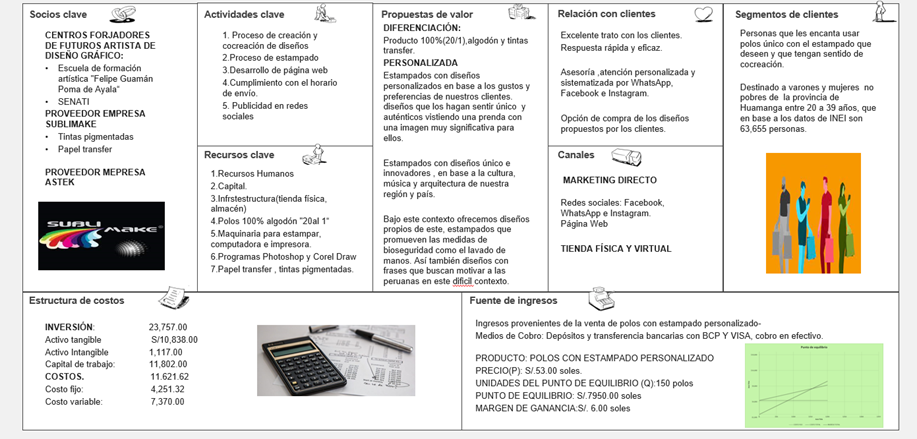
\includegraphics[scale=0.8]{Figuras/ModeloNegocioCANVAS.png}
\caption{Modelo de Negocio CANVAS}
\label{figura1}
\end{figure}
\end{landscape}

\newpage

\section{Estrategia empresarial}
\lhead[\thepage]{\thesection. Estrategia empresarial}

\subsection{Estrategia Organizacional}

\subsubsection{Misión}
Empresa dedicada a la comercialización de camisetas con estampados personalizados dirigidas a satisfacer las necesidades de los clientes exclusivos abarcando su estilo de ver y vivir la vida.
\subsubsection{Visión}

Convertirnos en una empresa reconocida en Ayacucho dentro del rubro de polos personalizados por la calidad de sus prendas y exclusividad en el diseño.
\subsubsection{Valores de la empresa.}

Los valores de nuestra empresa vinculan a los trabajadores, proveedores y clientes, crea un clima de respeto y mayor confianza fortaleciendo así la cultura organizacional que manejamos.
\begin{itemize}
\item Trabajo en equipo.
\item Confianza y compromiso.
\item Innovación y diversificación y creatividad
\item Orientación al cliente
\end{itemize}

\subsection{Objetivos de empresa}

\subsubsection{En el corto plazo (2021-2022)}
\begin{itemize}
\item Ofrecer servicios personalizados de diseño gráfico acorde a las exigencias de nuestros potenciales consumidores.
\item Lograr que nuestra marca sea reconocida en Facebook.
\item Elaborar un plan estratégico para la introducción de polos con motivos de los Carnavales, Semana Santa y el Bicentenario.
\end{itemize}

\subsubsection{En el mediano plazo (2022-2023)}
\begin{itemize}
\item Diseñar una plataforma digital donde el cliente pueda diseñar su polo y nuestra empresa encargarse de confeccionarlo.
\item Lograr distribuir nuestros polos a los distintos centros comerciales de la región.
\end{itemize}

\subsubsection{En el largo plazo (5 años)}
\begin{itemize}
\item Lograr distribuir nuestros polos a los distintos centros comerciales del Perú.
\item Contar con nuestra propia planta de confección de polos.
\item Asumir nuevas inversiones en nuestro rubro.
\end{itemize}

\subsection{Estrategia Genéricas de Porter}
La empresa adopta la estrategia del Océano Azul, se obtendrá una ventaja competitiva mediante la diferenciación y la segmentación.

\subsubsection{Estrategia de diferenciación}
Esta estrategia servirá para obtener la fidelización del cliente mediante la determinación de distintas características fuera de lo común como lo son las siguientes:
\paragraph{En el corto plazo:}
\begin{itemize}
\item Brindaremos un producto personalizado, con estampados únicos, con un material de calidad.
\item Innovaremos constantemente, y nos mantendremos en línea con las tendencias mundiales, así como con las tendencias temporales como lo son las estaciones del año y los eventos festivos como carnavales, semana santa, navidad, fiestas patrias, 14 de febrero, etc. satisfaciendo siempre los gustos y las expectativas de nuestros clientes.
\item Promoveremos las celebraciones familiares y las románticas como son los cumpleaños, aniversarios de parejas, etc.
\end{itemize}

\paragraph{En el mediano plazo:}
\begin{itemize}
\item Brindar asesoría y orientación mediante nuestras redes sociales acerca de los modelos que deseen nuestros clientes, para que de esta forma ellos puedan quedar plenamente satisfechos con el diseño elaborado.
\item Aprovecharemos las opiniones y sugerencias que nuestros clientes nos dejen en nuestras redes sociales y además también tendremos un buzón de sugerencias para nuestros trabajadores y de esta forma seguir mejorando en el servicio brindado.
\item Para llegar a las distintas partes de la región nos esmeraremos en crear buenos materiales y audio visuales.
\end{itemize}

\paragraph{En el largo plazo:}
\begin{itemize}
\item Seremos auspiciadores de distintos eventos, primero de eventos regionales y luego de eventos nacionales, esto para hacer más conocida nuestra marca.
\item Crearemos un ambiente de trabajo saludable para nuestros trabajadores y así poder empoderarlos y obtener una mayor productividad.
\end{itemize}

\subsubsection{Estrategia de Segmentación}
Nuestra segmentación estará enfocada en los jóvenes de entre 20 y 39 años.

\subsection{Estrategia Organizacional}
Para poder brindar asesorías personalizadas para mantener a nuestros clientes al tanto de la moda actual necesitamos contar con diversos factores críticos de éxito.

\subsubsection{Capital Humano}
\begin{itemize}
\item Contar con personal capacitado.
\item Asesorar a nuestras clientas en las nuevas tendencias, colores y consejos de moda que van con cada una de ellas, dependiendo del color de piel, las tallas, tamaño, color de cabello, etc.
\item Se utilizará la tercerización, es decir, que, tanto el contador y gerente de la empresa serán contratados mediante el servicio de tercerización del personal administrativo.
\end{itemize}

\subsubsection{Facilitadores tecnológicos.}
\begin{itemize}
\item Contar con una página web, donde se transmita al cliente que puede acceder a comprar nuestros productos por medio ella.
\item El acceso a internet nos proporcionará disponibilidad de modelos, pues podremos estar en frecuente visualización para ver las nuevas tendencias que aparecen en todo el mundo.
\item Las etiquetas y empaque y los polos serán comprados a otra empresa y no serán fabricados por StampAdek, esto nos permitirá aumentar la eficiencia y eficacia de la producción.
\end{itemize}

\subsubsection{Facilitadores organizacionales.}
\begin{itemize}
\item Compromiso con la aplicación de la estrategia de diferenciación.
\item Compromiso con nuevos proyectos para brindar nuevos servicios.
\end{itemize}

\subsection{Innovación del valor mediante la Matriz RICE:}
La siguiente matriz explica el medio o los puntos en los que se basan las estrategias descritas con anterioridad.

\subsection{Matriz Rice.}

\begin{table}[H] %Tabla con párrafo
\centering
\begin{tabular}{p{8cm}p{8cm}}
\hline
\textbf{Eliminar}                                                         & \textbf{Incrementar}                            \\
\hline %líneas horizontales%
Se eliminarán las barreras de la distancia.

Se eliminarán las tendencias establecidas ya que cada persona podrá diseñar su propia prenda, pero también se informará sobre la tendencia mundial.
                                                                          &     Se incrementará el asesoramiento y la atención personalizada.

El uso de las redes sociales como medio de comunicación con los clientes.                                                    \\
\hline
\textbf{Reducir}                                                          & \textbf{Crear}                                    \\
\hline 
Se reducirán las cantidades de polos con estampados con el mismo diseño.   &  Se creará polos con estampados y diseños personalizados, acorde al gusto de los clientes.                                                                                                                 \\
\hline
\end{tabular}
\caption{Matriz Rice}
\label{Tabla1}
\end{table}

\subsection{Estrategia Océano Azul.}
En el siguiente cuadro se realiza una breve diferenciación entre un negocio tradicional y nuestra empresa que adoptó la estrategia de Océano Azul.

\begin{table}[H] %Tabla con párrafo
\centering
\begin{tabular}{p{7cm}p{7cm}}
\hline
\textbf{Tiendas tradicionales}                                             & \textbf{STAMPADEK}                            \\
\hline %líneas horizontales%
Polos con diseños comunes y que no tienen un sentido específico.

Los clientes no participan en la creación de diseños.

Se realizan estampados, pero al por mayor y no en unidades.

No hacen uso de una plataforma de servicio al cliente.

                                                                          &     Polos con diseños que reflejen la identidad cultural.

Los clientes son creadores y cocreadores de los diseños.

Se realizan estampados personalizados y venta unitaria.

Se tendrá una plataforma de servicio al cliente.                                                                                \\
\hline
\end{tabular}
\caption{Estrategia de Océano Azul}
\label{Tabla2}
\end{table}

\subsection{Cadena de valor.}

\begin{figure}[h]
\centering
\raggedright
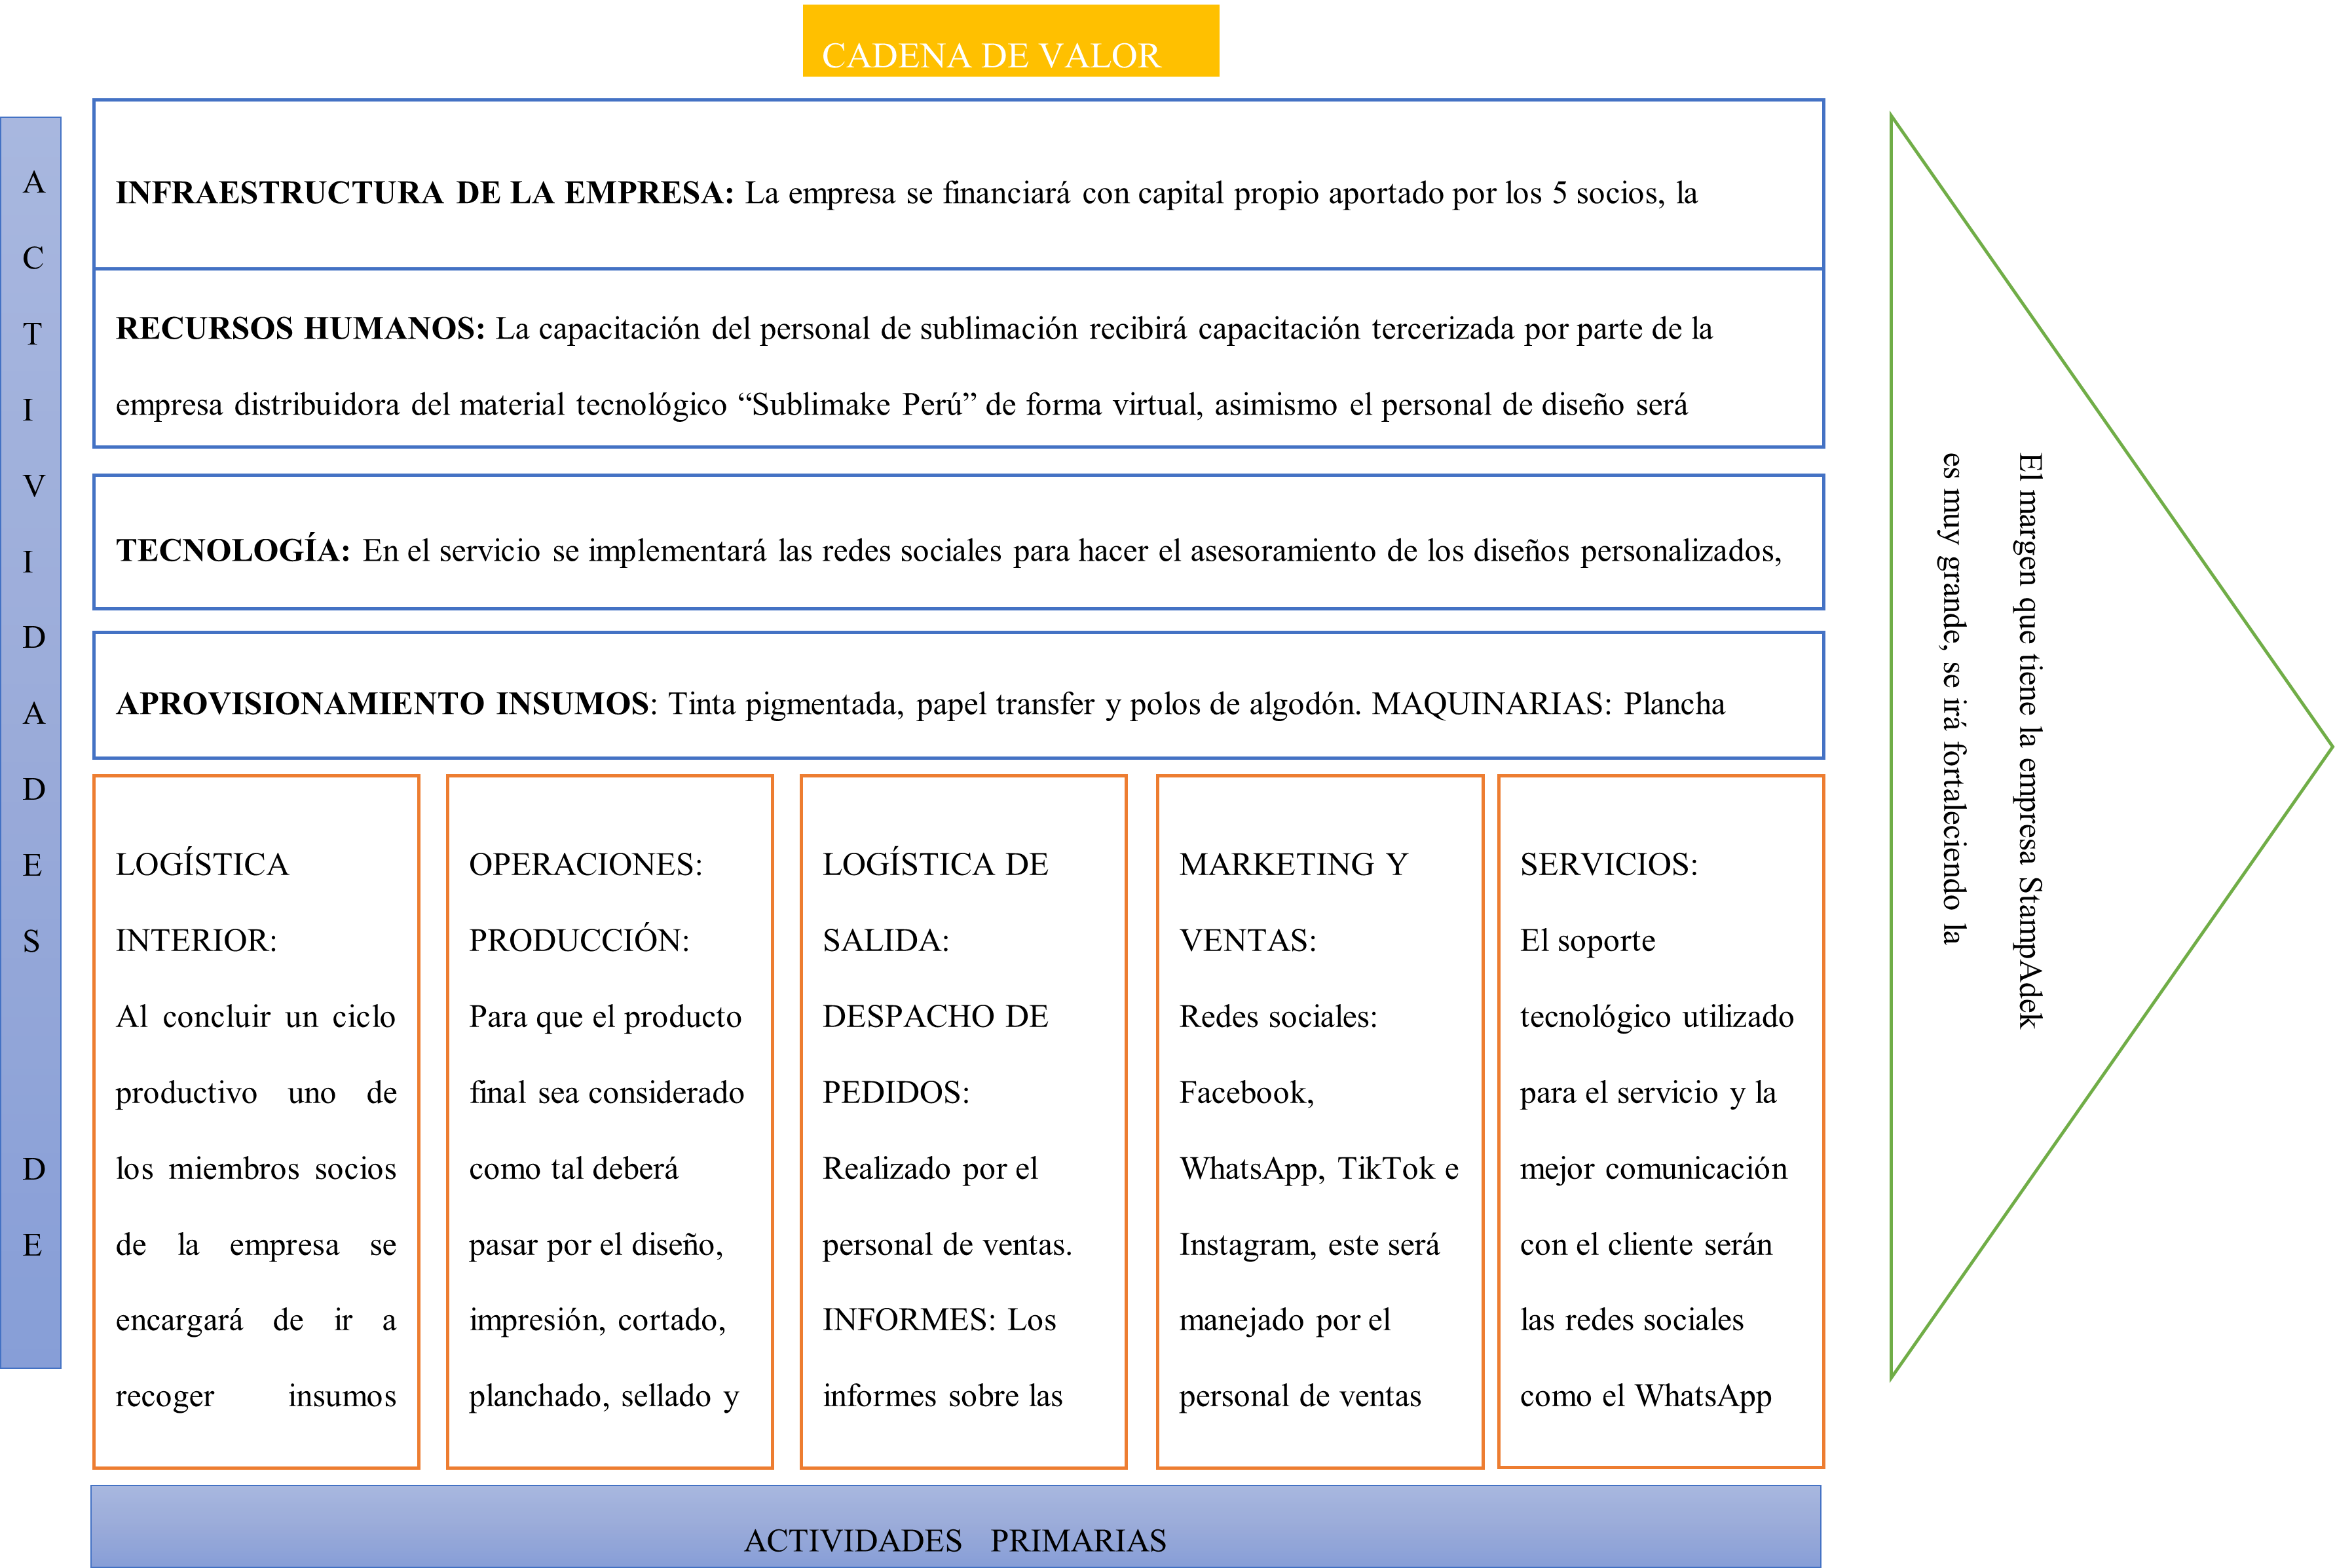
\includegraphics[scale=0.6]{Figuras/CadenaValor.png}
\caption{Cadena de Valor}
\label{figura1}
\end{figure}

\section{Modelo empresarial}
\lhead[\thepage]{\thesection. Modelo empresarial}

Nuestra empresa cuyo nombre comercial es “STAMP ADEK” estará definida como PERSONA JURÍDICA y será aperturada por: ALCA AYME, Yudith Carolina, ACHALMA MENDOZA Edison, GUTIÉRREZ LUCANA Diana y HUAMÁN CENTENO Kely y HUIZA QUISPE, Brenda Sofía, con lo cual podemos ejercer la actividad de estampado personalizado y venta de polos de algodón.

\subsection{Estructura societaria de la empresa}
El aspecto que tendrá nuestra empresa es de SOCIEDAD ANÓNIMA CERRADA (S.A.C.) que estará integrada por los 5 integrantes del grupo quienes seremos los socios, como tal está afecta a los siguientes requisitos:

\subsection{Constitución de la Empresa}
\begin{itemize}
\item Denominación Social: STAMP ADEK S.A.C.
\item Domicilio y plazo de funcionamiento: Jr. Asamblea 251 Stand No 148; con plazo indefinido.
\item Número de acciones: Estará conformado por 5 personas naturales. El proceso de formalización será el siguiente.
\item Búsqueda y reserva de nombre. Se debe realizar la búsqueda del nombre “STAMP ADEK S.A.C” en la SUNARP.
\item Elaboración de la Minuta de Constitución de la Empresa o Sociedad. A través de este documento el titular de la empresa o los miembros de la sociedad “STAMP ADEK S.A.C” manifiestan su voluntad de constituir la persona jurídica.
\item Aporte de capital. Podrá aportarse dinero o bienes (inmuebles o muebles, en estos últimos se entienden los derechos de crédito) los que se acreditarán con la inscripción de la transferencia a favor de la empresa o sociedad.
\item Elaboración de Escritura Pública ante el notario. Se generará la Escritura Pública de constitución de la empresa “STAMP ADEK S.A.C.
\item Inscripción de la empresa o sociedad en el Registro de Personas Jurídicas de la Sunarp. En la SUNARP obtendrá un asiento registral de inscripción de la empresa o sociedad como persona jurídica “STAMP ADEK S.A.C.”
\item Inscripción al RUC para Persona Jurídica. El RUC contiene los datos de identificación de las actividades económicas de “STAMP ADEK S.A.C.”. Registro de marca y logo. El registro de la marca tiene una vigencia de 10 años y un costo de 534,99 soles en el Banco de la Nación o Banco de Crédito usando el código 201000562.
\end{itemize}

\subsection{Licencia de funcionamiento}
El centro comercial VÍA 7 en el cual la empresa tendrá un stand ya cuenta con la licencia de funcionamiento.

\subsection{Tamaño de la empresa}
Nuestra empresa será constituida como una Microempresa debido a que cumplimos con los requisitos establecidos, registrando menos de los 150 UITs establecidos.

\subsection{Régimen Tributario}
De acuerdo con nuestra capacidad de producción lo cual influirá en las ventas se proyecta que nuestros ingresos serán de S/.120,120.00 anual lo cual equivale a 28 UIT que son menores a S/.525,000, por lo cual nos acogeremos al Régimen Especial Tributario.

\chapter{Inversión y valor de recupero}\label{cap.2}
\markboth{Inversión y valor de recupero}{Inversión y valor de recupero}

\section{Presupuesto de Inversión}
\lhead[\thepage]{\thesection. Presupuesto de Inversión}

La inversión inicial en activos será de S/. 11,955 y una inversión en capital de trabajo de S/. 11,811 lo cual detallaremos a continuación tanto en inversiones tangibles, intangibles y capital de trabajo.

\subsection{Activos Fijos}

\begin{table}[H]
\centering
\begin{tabular}{lcccc}
\hline
\textbf{Detalle de inversión}    & \textbf{Cantidad} & \textbf{Costo unitario} & \textbf{Costo total} & \textbf{Porcentaje} \\
\hline %líneas horizontales%
Computadora portátil laptop      &     2             &     1,899               &              3,798   & 31.77\% \\
Impresora                        &     1             &     1,559               &              1,559   & 13.04\% \\
Plancha plana(estampado)         &     1             &     1,500               &              1,500   & 12.55\% \\
Pistola etiquetadora Textil      &     1             &     27                  &              27      & 0.23\%  \\
Total                            &                   &	                       &             6,884    & 57.58\% \\
\hline
\end{tabular}
\caption{Inversiones en maquinaria y equipo de producción}
\label{Tabla3}
\end{table}

\begin{table}[H]
\centering
\begin{tabular}{lcccc}
\hline
\textbf{Detalle de inversión}    & \textbf{Cantidad} & \textbf{Costo unitario} & \textbf{Costo total} & \textbf{Porcentaje} \\
\hline %líneas horizontales%
Escritorio para computador       &     1             &     130                 &              130     & 1.09\% \\
Silla de escritorio              &     1             &     50                  &              50      & 0.48\% \\
Silla                            &     2             &     30                  &              60      & 0.50\% \\
Exhibidor de polos               &     1             &     220                 &              220     & 1.84\%  \\
Espejo para vestidor             &     1             &     15                  &              15      & 0.13\%  \\
Probador vestidor de metal       &     1             &     49                  &              49      & 0.41\%  \\
Cortina de vestidor de polos     &     1             &     30                  &              30      & 0.25\%  \\
Moto lineal (eléctrica)          &     1             &     3400                &              3400    & 28.44\%  \\
Total                            &                   &	                       &             3,954    & 33.07\% \\
\hline
\end{tabular}
\caption{Inversiones en muebles, enseres y equipos de administración}
\label{Tabla4}
\end{table}

\subsection{Inversión en Activos Intangibles}

\begin{table}[H]
\begin{tabular}{lcc}
\hline
\textbf{Detalle de inversión}    & \textbf{Costo}    &  \textbf{Porcentaje}    \\
\hline %líneas horizontales%
Registro de marca y logo         &     535           &      4.48\%             \\
Constitución de la empresa       &     477           &      3.99\%             \\
Capacitación al personal         &     60            &      0.50\%             \\
Inscripción en SUNARP            &     45            &      0.38\%             \\
Total, gastos preoperativos      &     1117          &      9.34\%             \\
\hline
\end{tabular}
\caption{Inversión en activos intangibles}
\label{Tabla5}
\end{table}


\subsection{Inversión en Capital de Trabajo}
El cálculo del capital de trabajo se realizó mediante el método del periodo de desfase. En el cual se consideró el total de costos operacionales menos la depreciación y amortización para hallar costo operacional.\\

Cálculo del capital de trabajo ICT= CO (COPD)\\
Total, costos operacionales =	11,802\\
(-) depreciación =	(353)\\
(-) amort. Diferidos =	(19)\\
(=) Costo operacional =	11,430\\
    COPD (Costo operacional diario) = 	COPA/30\\
COPD =	381.01\\
Capital de trabajo =	11,811\\

El proceso se inicia con el primer desembolso para cancelar los insumos de la operación y termina cuando se venden los insumos, transformados en productos terminados; es decir, se toma en cuenta el tiempo que transcurre a partir del momento que la empresa inicia sus actividades productivas hasta cuando se obtiene el valor por la venta de los polos personalizados.

\section{Horizonte de Evaluación}
\lhead[\thepage]{\thesection. Horizonte de Evaluación}

Se toma un horizonte de evaluación de 5 años en concordancia con el tiempo de vida útil del activo principal de nuestra empresa que es la Plancha Transfer.

\section{Valores de Recupero}
\lhead[\thepage]{\thesection. Valores de Recupero}

\subsection{Método Contable}
Teniendo en cuenta la vida útil de cada activo fijo, el tiempo de recupero de la inversión es de 5 años. El Horizonte de evaluación es de 5 años. \\
VR= Valor adquisitivo – Depreciación acumulada


\begin{table}[H]
\centering
\resizebox{18cm}{!} {
\begin{tabular}{p{5cm}p{1.8cm}p{1.8cm}p{2.2cm}p{2.2cm}p{2.2cm}p{2.2cm}}
\hline
\textbf{Detalle de inversión} & \textbf{Valor de compra} & \textbf{Vida útil años} & \textbf{Tasa de depreciación} & \textbf{Depreciación anual} & \textbf{Depreciación acumulada} & \textbf{Valor de recupero}\\
\hline %líneas horizontales%
Escritorio para computador    &     6884          &     130                 &              130     & 1.09\%  &              130     & 1.09\% \\
Silla de escritorio           &     3798          &     50                  &              50      & 0.48\%  &              50      & 0.48\% \\
Silla                         &     2             &     30                  &              60      & 0.50\%  &              60      & 0.50\% \\
Exhibidor de polos            &     1             &     220                 &              220     & 1.84\%  &              220     & 1.84\%  \\
Espejo para vestidor          &     1             &     15                  &              15      & 0.13\%  &              15      & 0.13\% \\
Probador vestidor de metal    &     1             &     49                  &              49      & 0.41\%  &              49      & 0.41\% \\
Cortina de vestidor de polos  &     1             &     30                  &              30      & 0.25\%  &              30      & 0.25\%\\
Moto lineal (eléctrica)       &     1             &     3400                &              3400    & 28.44\% &              3400    & 28.44\% \\
Total                         &                   &	                        &             3,954    & 33.07\% &             3,954    & 33.07\%\\
Escritorio para computador    &     6884          &     130                 &              130     & 1.09\%  &              130     & 1.09\% \\
Silla de escritorio           &     3798          &     50                  &              50      & 0.48\%  &              50      & 0.48\% \\
Silla                         &     2             &     30                  &              60      & 0.50\%  &              60      & 0.50\% \\
Exhibidor de polos            &     1             &     220                 &              220     & 1.84\%  &              220     & 1.84\%  \\
Espejo para vestidor          &     1             &     15                  &              15      & 0.13\%  &              15      & 0.13\% \\
Probador vestidor de metal    &     1             &     49                  &              49      & 0.41\%  &              49      & 0.41\% \\
Cortina de vestidor de polos  &     1             &     30                  &              30      & 0.25\%  &              30      & 0.25\%\\
Moto lineal (eléctrica)       &     1             &     3400                &              3400    & 28.44\% &              3400    & 28.44\% \\
\hline
\end{tabular}
}
\caption{Tabla de depreciaciones y valor de recupero}
\label{Tabla6}
\end{table}


\chapter{Presupuesto de ingresos y egreso}\label{cap.3}
\markboth{Presupuesto de ingresos y egreso}{Presupuesto de ingresos y egreso}

\section{Presupuesto de ventas}
\lhead[\thepage]{\thesection. Presupuesto de ventas}

\begin{table}[H]
\centering
\resizebox{18cm}{!} {
\begin{tabular}{ccccccccccccccc}
\hline
\textbf{Año} & \textbf{Valor unitario} & \textbf{Mes 1} & \textbf{Mes 2} & \textbf{Mes 3} & \textbf{Mes 4} & \textbf{Mes 5} & \textbf{Mes 6} & \textbf{Mes 7} & \textbf{Mes 8} & \textbf{Mes 9} & \textbf{Mes 10} & \textbf{Mes 11} & \textbf{Mes 12} & \textbf{Total} \\ \hline
1            & 45                      & 13500          & 15030          & 15255          & 15345          & 15930          & 19935          & 16380          & 18630          & 14130          & 19980           & 17280           & 15165           & 196560         \\
2            & 45                      & 17973          & 18219          & 18464          & 18709          & 18954          & 19199          & 19444          & 19689          & 19935          & 20180           & 20425           & 20670           & 231860         \\
3            & 45                      & 20915          & 21160          & 21405          & 21651          & 21896          & 22141          & 22386          & 22631          & 22876          & 23121           & 23366           & 23612           & 267160         \\
4            & 45                      & 23857          & 24102          & 24347          & 24592          & 24837          & 25082          & 25328          & 25573          & 25818          & 26063           & 26308           & 26553           & 302460         \\
5            & 45                      & 26798          & 27044          & 27289          & 27534          & 27779          & 28024          & 28269          & 28514          & 28760          & 29005           & 29250           & 29495           & 337761         \\ \hline
\end{tabular}
}
\caption{Proyección de ventas en Nuevos Soles}
\label{Tabla7}
\end{table}

\section{Presupuesto de costos y gasto}
\lhead[\thepage]{\thesection. Presupuesto de costos y gasto}

\begin{table}[H]
\centering
\resizebox{18cm}{!} {
\begin{tabular}{ccccccccccccccc}
\hline
\textbf{Año} & \textbf{Valor unitario} & \textbf{Mes 1} & \textbf{Mes 2} & \textbf{Mes 3} & \textbf{Mes 4} & \textbf{Mes 5} & \textbf{Mes 6} & \textbf{Mes 7} & \textbf{Mes 8} & \textbf{Mes 9} & \textbf{Mes 10} & \textbf{Mes 11} & \textbf{Mes 12} & \textbf{Total} \\ \hline
1            & 39                      & 11802          & 13140          & 13336          & 13415          & 13926          & 17428          & 14320          & 16287          & 12353          & 17467           & 15107           & 13258           & 171839         \\
2            & 39                      & 18293          & 18490          & 18726          & 18923          & 19159          & 19355          & 19552          & 19788          & 19985          & 20221           & 20418           & 20654           & 233564         \\
3            & 39                      & 20850          & 21086          & 21283          & 21480          & 21716          & 21913          & 22149          & 22345          & 22581          & 22778           & 23014           & 23211           & 264407         \\
4            & 39                      & 23447          & 23644          & 23840          & 24076          & 24273          & 24509          & 24706          & 24942          & 25139          & 25375           & 25571           & 25768           & 295289         \\
5            & 39                      & 26004          & 26201          & 26437          & 26633          & 26869          & 27066          & 27302          & 27499          & 27696          & 27932           & 28128           & 28364           & 326132         \\ \hline
\end{tabular}
}
\caption{Proyección de costos en nuevos soles}
\label{Tabla8}
\end{table}

\section{Costos Unitarios}
\lhead[\thepage]{\thesection. Costos Unitarios}

\begin{table}[H]
\centering
\begin{tabular}{lc}
\hline
\textbf{Costo   fijo}              & \textbf{Soles}   \\ \hline
Gastos de producción               & 248,66           \\
Gastos administrativos             & 2438,06          \\
Gastos de ventas                   & 1770,00          \\
\textbf{Costo   variable}          & \textbf{Soles}   \\
Materia   prima e insumos          & 5230,40          \\
Mano   de obra                     & 2115,00          \\
Costos   indirectos de fabricación &                  \\
\textbf{Total,   Costo Variable}   & \textbf{7345,40} \\
Nº   de polos de 300 Unid.         & 300              \\
Costo   fijo unitario (100\%)      & 14,86            \\
Costo   variable unitario          & 24,48            \\
Costo   total unitario             & 39,34            \\
\textbf{Total, Costo Fijo}         & \textbf{4456,71} \\ \hline
\end{tabular}
\caption{Costo unitario lote 300 polos.}
\label{Tabla9}
\end{table}


\section{Estado de Resultados}
\lhead[\thepage]{\thesection. Estado de Resultados}

\begin{table}[H]
\centering
\resizebox{16cm}{!} {
\begin{tabular}{lccccc}
\hline
\multicolumn{1}{c}{\textbf{Rubro}}   & \textbf{Año 1}     & \textbf{Año 2}     & \textbf{Año 3}     & \textbf{Año 4}     & \textbf{Año 5}     \\ \hline
\textbf{Ingreso por ventas}          & \textbf{196560.00} & \textbf{231860.14} & \textbf{267160.28} & \textbf{302460.42} & \textbf{337760.56} \\
Cantidad                             & 4368.00            & 5152.45            & 5936.90            & 6721.34            & 7505.79            \\
Precio                               & 45.00              & 45.00              & 45.00              & 45.00              & 45.00              \\
\textbf{Costo de ventas}             & \textbf{4237.18}   & \textbf{4237.18}   & \textbf{4237.18}   & \textbf{4237.18}   & \textbf{4237.18}   \\
\textbf{Costos de producción}        & \textbf{106949.02} & \textbf{126155.96} & \textbf{145362.90} & \textbf{164569.83} & \textbf{183776.77} \\
Depreciación de activos   fijos      & 4237.18            & 4237.18            & 4237.18            & 4237.18            & 4237.18            \\
\textbf{Utilidad Bruta}              & \textbf{85373.80}  & \textbf{101467.00} & \textbf{117560.21} & \textbf{133653.41} & \textbf{149746.61} \\
\textbf{Gastos Operativos}           & \textbf{}          & \textbf{}          & \textbf{}          & \textbf{}          & \textbf{}          \\
Gastos de venta                      & 21420.00           & 21420.00           & 21420.00           & 21420.00           & 21420.00           \\
Gastos de administración             & 27600.00           & 27600.00           & 27600.00           & 27600.00           & 27600.00           \\
Amortización de intangibles          & 223.40             & 223.40             & 223.40             & 223.40             & 223.40             \\
\textbf{Utilidad operativa}          & \textbf{36130.40}  & \textbf{52223.60}  & \textbf{68316.81}  & \textbf{84410.01}  & \textbf{100503.21} \\
Intereses                            &                    &                    &                    &                    &                    \\
\textbf{Utilidad antes de Impuestos} & \textbf{36130.40}  & \textbf{52223.60}  & \textbf{68316.81}  & \textbf{84410.01}  & \textbf{100503.21} \\
Impuesto a la renta                  & 541.96             & 783.35             & 1024.75            & 1266.15            & 1507.55            \\
\textbf{Utilidad Neta}               & \textbf{35588.45}  & \textbf{51440.25}  & \textbf{67292.06}  & \textbf{83143.86}  & \textbf{98995.67}  \\ \hline
\end{tabular}
}
\caption{Proyección del estado de resultados para 5 años}
\label{Tabla10}
\end{table}

\section{Punto de Equilibrio}
\lhead[\thepage]{\thesection. Punto de Equilibrio}

El punto de equilibrio que presenta STAMPADEK es de S/. 156.00 unidades de polos y unas ventas de S/. 8.283.00 soles. Por debajo de S/. 156.00 unidades la empresa presentará pérdidas, debido a que los costos serían mayores que los ingresos. Por encima de S/. 156.00 unidades se presentan utilidades debido a que los ingresos son mayores que los costes. El precio de venta es de S/. 53.00 soles y el costo variable unitario es de 24.48.

\begin{figure}[h]
\centering
\raggedright
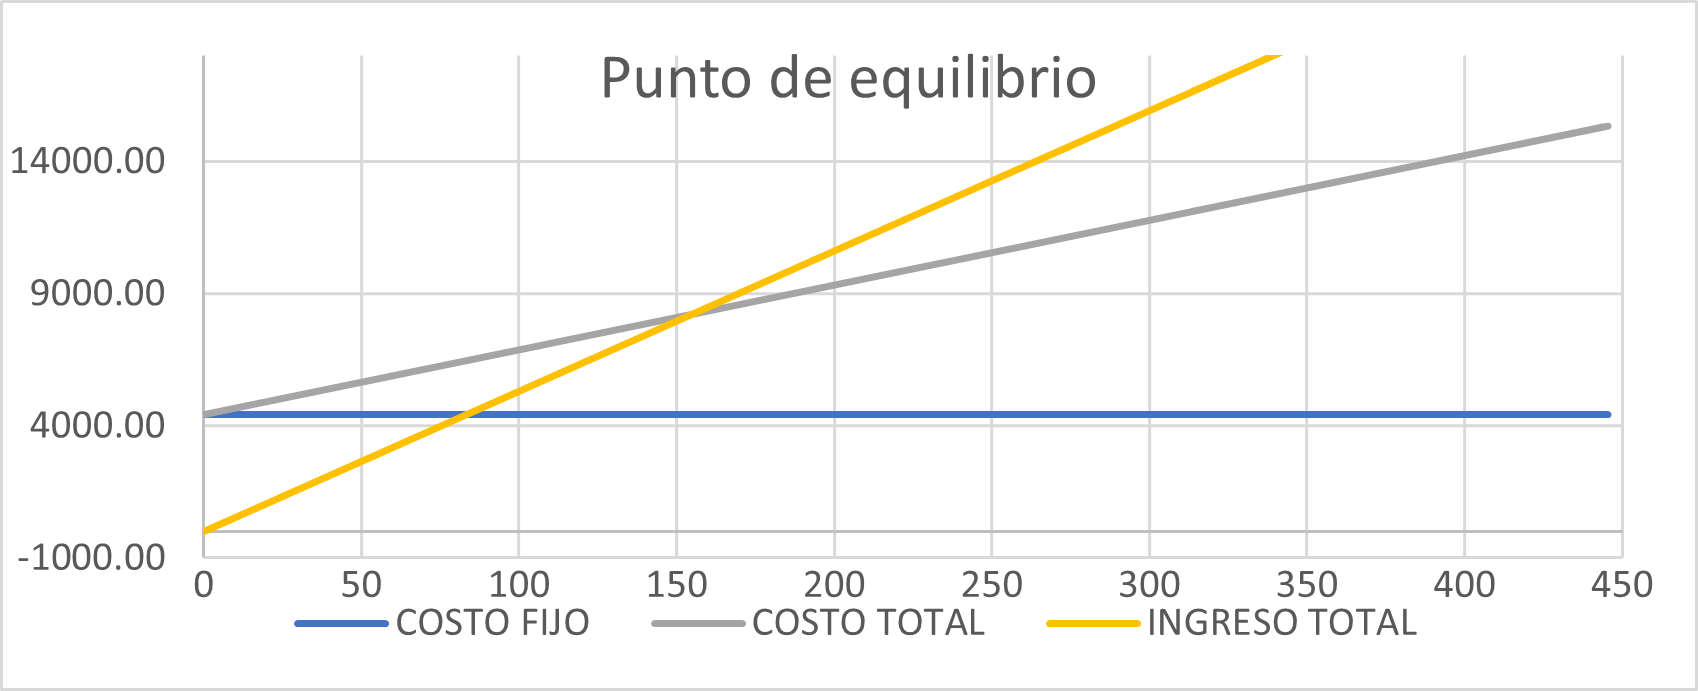
\includegraphics[scale=1.2]{Figuras/PuntoEquilibrio.png}
\caption{Punto de equilibrio de la empresa STAMPADEK}
\label{figura4}
\end{figure}


\chapter{Financiamiento y Costo de Capital}\label{cap.4}
\markboth{Financiamiento y Costo de Capital}{Financiamiento y Costo de Capital}

\section{Fuentes de Financiamiento}
\lhead[\thepage]{\thesection. Fuentes de Financiamiento}

El financiamiento para el proyecto STAMP ADEK estará conformado por 24\% (S/.5,766) con recursos propios de los socios, y el 76\% (S/.18,000) estará cubierto de un préstamo otorgado por la Cooperativa Santa María Magdalena a nombre del padre de una las socias bajo la modalidad de crédito personal.

\begin{table}[H]
\centering
\begin{tabular}{lcc}
\hline
\multicolumn{1}{c}{\textbf{Aportantes}} & \textbf{Monto}   & \textbf{\%}   \\ \hline
Edison   Achalma                        & S/.1,000         & 4\%           \\
Diana   Gutiérrez                       & S/.1,000         & 4\%           \\
Brenda   Huiza                          & S/.1,782         & 7\%           \\
Carolina   Alca                         & S/.1,000         & 4\%           \\
Kely   Huamán                           & S/.1,000         & 4\%           \\ \hline
\textbf{Total}                          & \textbf{\$5,766} & \textbf{24\%} \\ \hline
\end{tabular}
\caption{Capital propio}
\label{Tabla11}
\end{table}

\section{Financiamiento de Terceros}
\lhead[\thepage]{\thesection. Financiamiento de Terceros}

El crédito para nuestro para nuestra inversión inicial nos lo otorgará la Cooperativa Santa María Magdalena, a nombre del padre de una de nuestras accionistas. El producto del crédito es Credi-personal, el plazo para pagar la deuda es de 3 años, el método aplicado por la Cooperativa es el francés ya que pagaremos una cuota constante de S/.647.34 y un interés total de S/. 5304.15. El préstamo se solicitará el 2 de agosto del 2021.

% Please add the following required packages to your document preamble:
% \usepackage[table,xcdraw]{xcolor}
% If you use beamer only pass "xcolor=table" option, i.e. \documentclass[xcolor=table]{beamer}
\begin{table}[H]
\begin{tabular}{ll}
Préstamo                     & S/.18,000.00 \\
\rowcolor[HTML]{F2F2F2} 
Moneda                       & Soles        \\
Número de cuotas             & 36           \\
\rowcolor[HTML]{F2F2F2} 
Periodo de pago              & Mensual      \\
TEA nominal (i)              & 21.50\%      \\
\rowcolor[HTML]{F2F2F2} 
TEM (nominal)                & 1.64\%       \\
Inflación anual (proyectado) & 2.00\%       \\
\rowcolor[HTML]{F2F2F2} 
Inflación mensual            & 0.17\%       \\
TEM (real)                   & 1.47\%       \\
\rowcolor[HTML]{F2F2F2} 
Cuota                        & S/.647.34    \\
Monto del préstamo           & S/.18,000.00
\end{tabular}
\end{table}

\begin{table}[H]
\begin{tabular}{lcccccc}
\hline
\multicolumn{1}{c}{\textbf{N°}} & \textbf{Fecha} & \textbf{Monto} & \textbf{Interés} & \textbf{Amortización} & \textbf{Cuota} & \textbf{Saldo final} \\ \hline
                                & 08/2/2021      & 18000.00       & 0.00             & 0.00                  & 0.00           & 18000.00             \\
1                               & 09/1/2021      & 18000.00       & 264.33           & 383.00                & 647.34         & 17617.00             \\
2                               & 10/1/2021      & 17617.00       & 258.71           & 388.63                & 647.34         & 17228.37             \\
3                               & 10/31/2021     & 17228.37       & 253.00           & 394.33                & 647.34         & 16834.03             \\
4                               & 11/30/2021     & 16834.03       & 247.21           & 400.13                & 647.34         & 16433.91             \\
5                               & 12/30/2021     & 16433.91       & 241.34           & 406.00                & 647.34         & 16027.91             \\
6                               & 01/29/2022     & 16027.91       & 235.37           & 411.96                & 647.34         & 15615.94             \\
7                               & 02/28/2022     & 15615.94       & 229.32           & 418.01                & 647.34         & 15197.93             \\
8                               & 03/30/2022     & 15197.93       & 223.19           & 424.15                & 647.34         & 14773.78             \\
9                               & 04/29/2022     & 14773.78       & 216.96           & 430.38                & 647.34         & 14343.40             \\
10                              & 05/29/2022     & 14343.40       & 210.64           & 436.70                & 647.34         & 13906.69             \\
11                              & 06/28/2022     & 13906.69       & 204.22           & 443.11                & 647.34         & 13463.58             \\
12                              & 07/28/2022     & 13463.58       & 197.72           & 449.62                & 647.34         & 13013.96             \\
13                              & 08/27/2022     & 13013.96       & 191.11           & 456.22                & 647.34         & 12557.73             \\
14                              & 09/26/2022     & 12557.73       & 184.41           & 462.92                & 647.34         & 12094.81             \\
15                              & 10/26/2022     & 12094.81       & 177.62           & 469.72                & 647.34         & 11625.09             \\
16                              & 11/25/2022     & 11625.09       & 170.72           & 476.62                & 647.34         & 11148.47             \\
17                              & 12/25/2022     & 11148.47       & 163.72           & 483.62                & 647.34         & 10664.85             \\
18                              & 01/24/2023     & 10664.85       & 156.62           & 490.72                & 647.34         & 10174.12             \\
19                              & 02/23/2023     & 10174.12       & 149.41           & 497.93                & 647.34         & 9676.20              \\
20                              & 03/25/2023     & 9676.20        & 142.10           & 505.24                & 647.34         & 9170.96              \\
21                              & 04/24/2023     & 9170.96        & 134.68           & 512.66                & 647.34         & 8658.30              \\
22                              & 05/24/2023     & 8658.30        & 127.15           & 520.19                & 647.34         & 8138.11              \\
23                              & 6/23/2023      & 8138.11        & 119.51           & 527.83                & 647.34         & 7610.28              \\
24                              & 07/23/2023     & 7610.28        & 111.76           & 535.58                & 647.34         & 7074.70              \\
25                              & 08/22/2023     & 7074.70        & 103.89           & 543.44                & 647.34         & 6531.26             
\end{tabular}
\end{table}

\begin{table}[]
\begin{tabular}{ccccccc}
\hline
\textbf{N°} & \textbf{Fecha} & \textbf{Monto} & \textbf{Interés} & \textbf{Amortización} & \textbf{Cuota} & \textbf{Saldo final} \\ \hline
26          & 09/21/2023     & 6531.26        & 95.91            & 551.42                & 647.34         & 5979.83              \\
27          & 10/21/2023     & 5979.83        & 87.82            & 559.52                & 647.34         & 5420.31              \\
28          & 11/20/2023     & 5420.31        & 79.60            & 567.74                & 647.34         & 4852.57              \\
29          & 12/20/2023     & 4852.57        & 71.26            & 576.08                & 647.34         & 4276.50              \\
30          & 01/19/2024     & 4276.50        & 62.80            & 584.54                & 647.34         & 3691.96              \\
31          & 02/18/2024     & 3691.96        & 54.22            & 593.12                & 647.34         & 3098.84              \\
32          & 03/19/2024     & 3098.84        & 45.51            & 601.83                & 647.34         & 2497.01              \\
33          & 04/18/2024     & 2497.01        & 36.67            & 610.67                & 647.34         & 1886.34              \\
34          & 05/18/2024     & 1886.34        & 27.70            & 619.64                & 647.34         & 1266.70              \\
35          & 06/17/2024     & 1266.70        & 18.60            & 628.74                & 647.34         & 637.97               \\
36          & 07/17/2024     & 637.97         & 9.37             & 637.97                & 647.34         & 0.00                 \\ \hline
\textbf{}   & \textbf{Total} & \textbf{}      & \textbf{5304.15} & \textbf{18000.00}     & \textbf{}      & \textbf{}            \\ \hline
\end{tabular}
\caption{Amortización de la Deuda, Método Francés}
\label{Tabla12}
\end{table}

\section{Costos de Capital Propio (COK)}
\lhead[\thepage]{\thesection. Costos de Capital Propio (COK)}

El Beta total de Mercados Emergentes des apalancado para procesamiento de vestidos de 3.50, es decir la cantidad de riesgo operativo como financiero, que soportan las acciones con respecto al portafolio de mercado.
Después del análisis se obtuvo una tasa de descuento COK de 22.92\%, que es el porcentaje mínimo que espera recibir el accionista por su inversión.
\begin{equation}
•Kurt=Rf usa+Bu totalME*(Rm-Rf)usa+Rp Peru
\end{equation}

Donde:							

\begin{table}[H]
\begin{tabular}{lll}
Rf usa =        & 4.95\% & Promedio geométrico 1928-2020 *los últimos 30 años         \\
Bu total ME   = & 3.50   & Beta total des apalancado para   procesamiento de vestidos \\
(Rm-Rf) =       & 4.64\% & promedio geométrico   1928-2020 *los últimos 30 años       \\
Rp =            & 1.30\% & Promedio 2020                                              \\
Kurt =          & 22.4\% & COK des apalancado con   Riesgo Total                     
\end{tabular}
\end{table}


\section{Costos de Capital Promedio Ponderado (KWACC)}
\lhead[\thepage]{\thesection. Costos de Capital Promedio Ponderado (KWACC)}

Dado la combinación del capital propio con un monto en porcentajes de 24.0\% con un capital financiado por tercero de 76.0\% Procedemos a la determinación ponderada de participación. Como se puede observar en el gráfica el valor del costo de capital ponderado es de 21.5\%.

\begin{equation}
•Kwac rt=E/V*Kert+D/V*Kd*(1-t)
\end{equation}

Donde:

\begin{table}[H]
\begin{tabular}{cll}
E/V* =  & 24.0\% & Combinación del capital propio       \\
Kert =  & 21.1\% & Costo de capital propio   apalancado \\
D/V* =  & 76.0\% &                                      \\
Kd =    & 21.0\% & Costo de la deuda                    \\
T       & 1.5\%  & Tasa de impuesto a la   renta        \\
Kwacc = & 21.5\% &                                     
\end{tabular}
\end{table}


\chapter{Rentabilidad del proyecto}\label{cap.5}
\markboth{Rentabilidad del proyecto}{Rentabilidad del proyecto}

\section{Premisas}
\lhead[\thepage]{\thesection. Premisas}

El horizonte de evaluación del proyecto es de 5 años, el precio de venta de nuestros polos es de 53 soles, y el coste de oportunidad es de 12% nominal anual y la TEA es de 21.50%.
El capital de trabajo se realiza con el método de déficit acumulado máximo, se calcularon las depreciaciones de los activos y se estimó el valor de recupero con el método contable. El flujo de caja está proyectado en términos reales, la realización de la compra de nuestra materia prima y la venta de nuestro producto es al contado, y no se cuenta con stock de inventarios en productos tanto como en materia prima.


\section{Flujo de caja Económico y Financiero}
\lhead[\thepage]{\thesection. Flujo de caja Económico y Financiero}

\begin{table}[H]
\centering
\resizebox{16.5cm}{!} {
\begin{tabular}{lcccccc}
\hline
\multicolumn{1}{c}{\textbf{Rubro}} & \textbf{Año 0} & \textbf{Año 1} & \textbf{Año 2} & \textbf{Año 3} & \textbf{Año 4} & \textbf{Año 5} \\ \hline
Flujo de inversión y Liquidación   &                &                &                &                &                &                \\
Activo fijo tangible               & -10838.00      & -15.00         & -5372.00       & -3415.00       & -5372.00       & -15.00         \\
Activo fijo intangible             & -1116.99       &                &                &                &                &                \\
Capital de trabajo                 & -12336.33      & -2215.48       & -2215.48       & -2215.48       & -2215.48       & 0.00           \\
Recupero capital de trabajo        &                &                &                &                &                & 21198.24       \\
Recupero activo fijo tangible      &                &                &                &                &                & 3826.12        \\
Flujo de inversión y liquidación   & -24291.32      & -2230.48       & -7587.48       & -5630.48       & -7587.48       & 25009.36       \\
Flujo de Caja Operativo            &                &                &                &                &                &                \\
Ingreso por ventas                 &                & 196560.00      & 231860.14      & 267160.28      & 302460.42      & 337760.56      \\
Costos de producción               &                & -106949.02     & -126155.96     & -145362.90     & -164569.83     & -183776.77     \\
Gastos de venta                    &                & -21420.00      & -21420.00      & -21420.00      & -21420.00      & -21420.00      \\
Gastos de administración           &                & -27600.00      & -27600.00      & -27600.00      & -27600.00      & -27600.00      \\
Pago de IGV                        &                & -32501.31      & -38855.33      & -45209.36      & -51563.38      & -57917.41      \\
Impuestos                          &                & -541.96        & -783.35        & -1024.75       & -1266.15       & -1507.55       \\
Total Flujo de Caja Operativo      & 0.00           & 7547.71        & 17045.49       & 26543.27       & 36041.05       & 45538.83       \\
Flujo de Caja económico FCE        & -24291.32      & 5317.23        & 9458.01        & 20912.79       & 28453.57       & 70548.19       \\ \hline
\end{tabular}
}
\caption{Flujo de caja real de la empresa StampAdek de polos personalizados}
\label{Tabla13}
\end{table}

Este flujo de caja toma en cuenta solo el dinero con el que se ha financiado la empresa StampAdek, más no toma el financiamiento de la inversión por entidades financieras u otros. Se observa que el Flujo de Caja Económico es rentable positivo desde el primer año, esto significa que el proyecto es rentable por sí mismo.

\section{Evaluación Económica y Financiera}
\lhead[\thepage]{\thesection. Evaluación Económica y Financiera}

Para realizar nuestra evaluación económica, requeriremos de los métodos que nos ayudará a determinar la rentabilidad del proyecto para ello hallarnos los indicadores correspondientes, en primer lugar, determinaremos el valor actual neto económico (VANE), donde tomaremos en cuenta los flujos caja económica, la tasa de capital propio y calcularemos median la formula
\begin{equation}
•\sum^{N}_{t=1}F_{t}\div(1+k)^{t} - I_{0}
\end{equation}
dado el cálculo, nuestro VANE es igual a 35973.95. Este valor nos muestra que nuestro proyecto es rentable ya que el valor es positivo y cumple con las mínimas condiciones establecidas. 

\begin{table}[H]
\begin{tabular}{lll}
\textbf{VANE}  & \textbf{35973.95} & \textbf{Soles}                                   \\
FCEt &          & flujo de caja económica e el periodo   t        \\
Ku   & 22.47\%  & costo de capital propio des apalancado          \\
Io   & 24291.32 & inversión total en el periodo cero              \\
t    & 5        & periodo de tiempo                               \\
n    & 5        & periodo de horizonte de evaluación del proyecto
\end{tabular}
\caption{Cálculo del Valor Actual Neto Económico.}
\label{Tabla14}
\end{table}

\subsection{Tasas Interna de Retorno (TIRE)}

Este valor se expresará en términos de porcentual es cuando VANE es igual a cero, este valor nos muestra el máximo rendimiento que se obtendrá sobre la inversión total, para determinar dicho valor debemos remplazar los valores en la siguiente formula

\begin{equation}
•0=\sum^{N}_{t=1}F_{t}\div(1+k)^{t} - I_{0}
\end{equation}
 
Este indicador representa el máximo retorno que los flujos puedan otorgarnos sobre la inversión total. Realizando el cálculo nuestro TIRE es de 57.79\%   dado este valor podemos afirmar que nuestro proyecto es rentable. 

\begin{table}[H]
\begin{tabular}{lclllll}
\textbf{TIRE} & \multicolumn{1}{l}{\textbf{57.79\%}} & \multicolumn{5}{l}{\textbf{Promedio   anual}}                      \\
FCEt          &                                      & \multicolumn{5}{l}{flujo de caja economica e el periodo t}         \\
Ku            & 22.47\%                              & \multicolumn{5}{l}{costo de capital propio des apalancado}         \\
Io            & 24291.32                             & \multicolumn{5}{l}{inversion total en el periodo cero}             \\
t             & 5                                    & \multicolumn{5}{l}{periodo de tiempo}                              \\
n             & 5                                    & \multicolumn{5}{l}{periodo de horizonte de evalucion del proyecto} \\
              &                                      & \multicolumn{5}{l}{}                                               \\
\textbf{PEC}  & \multicolumn{1}{l}{\textbf{215}}     & \multicolumn{5}{l}{Unidad/periodo}                                
\end{tabular}
\caption{Cálculo de la Tasa Interna de Retorno económico}
\label{Tabla15}
\end{table}

\subsection{Valor actual neto financiero (VANF)}
Este método de evaluación nos mide las ganancias o pérdidas en términos de flujo financiero, para determinar este valor requeriremos del flujo de caja financiera y del flujo de la caja de la deuda y la KWACC . Este indicador nos mostrará el valor del negocio en términos monetarios.  Para determinar el valor remplazamos los valores en la siguiente formula 

\begin{equation}
•\sum^{N}_{t=1}F_{t}\div(1+k)^{t} - I_{0}+D
\end{equation}

Calculando el valor, nuestro VANF es de 53907.87 dando lugar a una rentabilidad financiera. 

\begin{table}[H]
\begin{tabular}{lclllll}
\textbf{VANF} & \multicolumn{1}{l}{\textbf{53907.87}} & \multicolumn{5}{l}{\textbf{}}                                      \\
FCFt          &                                       & \multicolumn{5}{l}{Flujo de caja financiero del periodo}           \\
Kwacc         & 21.53\%                               & \multicolumn{5}{l}{costo de capital propio apalancado}             \\
D             & 18000.00                              & \multicolumn{5}{l}{Monto de la deuda}                              \\
Io            & -6291.32                              & \multicolumn{5}{l}{Inversion inicial total}                        \\
n             & 5                                     & \multicolumn{5}{l}{periodo de horizonte de evalucion del proyecto} \\
\textbf{PEC}  & \multicolumn{1}{l}{\textbf{215}}      & \multicolumn{5}{l}{Unidad/periodo}                                
\end{tabular}
\caption{Cálculo del Valor Actual Neto Financiero}
\label{Tabla16}
\end{table}

\subsection{Tasa Interna de Retorno Financiera (TIRF)}
La TIRF es una tasa que expresa en términos porcentuales cuando nuestra VANF es igual a 0, esta tasa nos refleja el rendimiento promedio que se obtendrá sobre la inversión. Para calcular esta tasa remplazaremos la Kwacc, deuda e inversión en la siguiente formula

\begin{equation}
•0=\sum^{N}_{t=1}F_{t}\div(1+k)^{t} - I_{0}+D
\end{equation}
 
 Dado el cálculo nuestro TIRF es de 76.57\%   Este valor nos indica que nuestro proyecto incrementara el patrimonio o inversión aportada por acciones. 
 
\begin{table}[H]
\begin{tabular}{lclllll}
\textbf{TIRF} & \multicolumn{1}{l}{\textbf{76.57\%}} & \multicolumn{5}{l}{\textbf{}}                            \\
VANF          & 0                                    & \multicolumn{5}{c}{}                                     \\
FCFt          & 99790.18                             & \multicolumn{5}{l}{Flujo de caja financiero del periodo} \\
Kwacc         & 21.53\%                              & \multicolumn{5}{l}{costo de capital propio apalancado}   \\
D             & 18000.00                             & \multicolumn{5}{l}{Monto de la deuda}                    \\
Io            & -6291.32                             & \multicolumn{5}{l}{Inversion inicial total}              \\
\textbf{PEC}  & \multicolumn{1}{l}{\textbf{215}}     & \multicolumn{5}{l}{Unidad/periodo}                      
\end{tabular}
\caption{Cálculo de la Tasa Interna de Retorno Financiera}
\label{Tabla17}
\end{table}
 

\section{Análisis de Sensibilidad y Escenarios}
\lhead[\thepage]{\thesection. Análisis de Sensibilidad y Escenarios}

\begin{table}[H]
\begin{tabular}{lc}
\textbf{Activo Fijo}       & \textbf{11954.99} \\
Capital de Trabajo         & 12336.33          \\
Vida útil                  & 5                 \\
Cantidad de ventas   año 1 & 4368              \\
Precio                     & 45                \\
tasa   crecimiento         &                   \\
\textbf{Materia prima}     & \textbf{17.43}    \\
Mano de obra               & 7.05              \\
costo variable   unitario  & 24.480            \\
Costo fijo total           & 4411.71           \\
Tasa de   impuesto         & 1.5\%             \\
COK = Ku                   & 22.47\%           \\
Kwacc                      & 21.53\%           \\
Kwacc                      & 21.53\%          
\end{tabular}
\caption{Principales Datos del Análisis Contable}
\label{Tabla18}
\end{table}


\subsection{Análisis de los Puntos Críticos}

% Please add the following required packages to your document preamble:
% \usepackage[table,xcdraw]{xcolor}
% If you use beamer only pass "xcolor=table" option, i.e. \documentclass[xcolor=table]{beamer}
\begin{table}[H]
\begin{tabular}{lclll}
\multicolumn{5}{c}{\cellcolor[HTML]{1D6194}{\color[HTML]{FFFFFF} \textbf{1.-   ANÁLISIS DE PUNTOS CRÍTICOS}}}                                                                                             \\
\multicolumn{3}{l}{{\color[HTML]{FF0000} ¿Qué precio debe tener el produccto para que  el VANE=0?}} &                                                                             &                       \\
\textbf{Variable}         & \multicolumn{1}{l}{\textbf{Valor Actual}} & \textbf{Valor Marginal}     & \textbf{Soporte \%}                                                         &                       \\
Precio                    & 45.00                                     & \multicolumn{1}{c}{42.74}   & \multicolumn{1}{c}{\cellcolor[HTML]{FFC7CE}{\color[HTML]{9C0006} -5.02\%}}  & \multicolumn{1}{c}{2} \\
Tasa Crec.                & 15\%                                      & \multicolumn{1}{c}{3.62\%}  & \multicolumn{1}{c}{\cellcolor[HTML]{FFC7CE}{\color[HTML]{9C0006} -75.06\%}} & \multicolumn{1}{c}{}  \\
\textbf{Precio MP}        & \textbf{17.43}                            & \multicolumn{1}{c}{19.69}   & \multicolumn{1}{c}{\cellcolor[HTML]{C6EFCE}{\color[HTML]{006100} 12.97\%}}  & \multicolumn{1}{c}{3} \\
Costo MO                  & 7.05                                      & \multicolumn{1}{c}{9.31}    & \multicolumn{1}{c}{\cellcolor[HTML]{C6EFCE}{\color[HTML]{006100} 32.07\%}}  & \multicolumn{1}{c}{4} \\
Cantidad de ventas año 1  & 4368.00                                   & \multicolumn{1}{c}{2216.44} & \multicolumn{1}{c}{\cellcolor[HTML]{FFC7CE}{\color[HTML]{9C0006} -49.26\%}} & \multicolumn{1}{c}{1} \\
Costo fijo total          & 4411.71                                   &                             &                                                                             &                       \\
Tasa de   impuesto        & 1.5\%                                     &                             &                                                                             &                       \\
COK = Ku                  & 22.47\%                                   &                             &                                                                             &                       \\
Kwacc                     & 21.53\%                                   &                             &                                                                             &                       \\
Kwacc                     & 21.53\%                                   &                             &                                                                             &                      
\end{tabular}
\caption{Análisis de los Puntos Críticos}
\label{Tabla19}
\end{table}

\subsection{Análisis de Sensibilidad Unidimensional }
¿Cómo varia el VANE, TIRE y PEC al modificarse el precio del producto?

% Please add the following required packages to your document preamble:
% \usepackage[table,xcdraw]{xcolor}
% If you use beamer only pass "xcolor=table" option, i.e. \documentclass[xcolor=table]{beamer}
\begin{table}[H]
\begin{tabular}{lcccc}
                                                   & \multicolumn{1}{l}{}              & \multicolumn{3}{c}{\cellcolor[HTML]{1D6194}{\color[HTML]{FFFFFF} \textbf{RESULTADOS}}}                               \\
\multicolumn{1}{c}{}                               & \cellcolor[HTML]{D9D9D9}\textbf{} & \cellcolor[HTML]{D9D9D9}\textbf{TIRE} & \cellcolor[HTML]{D9D9D9}\textbf{VANE} & \cellcolor[HTML]{D9D9D9}\textbf{PEC} \\
\cellcolor[HTML]{75BDA7}                           & \textbf{BASE}                     & \textbf{58\%}                         & \textbf{36048.35}                     & \textbf{215.00}                      \\
\cellcolor[HTML]{75BDA7}                           & \cellcolor[HTML]{FFFF00}42.74     & 22\%                                  & \textbf{0.00}                         & 241.62                               \\
\cellcolor[HTML]{75BDA7}                           & 43.00                             & 27\%                                  & 4160.29                               & 238.21                               \\
\cellcolor[HTML]{75BDA7}                           & 44.00                             & 42\%                                  & 20104.32                              & 226.01                               \\
\rowcolor[HTML]{ABD8CA} 
\multicolumn{1}{c}{\cellcolor[HTML]{75BDA7}PRECIO} & \textbf{45.00}                    & \textbf{58\%}                         & \textbf{36048.35}                     & \textbf{215.00}                      \\
\cellcolor[HTML]{75BDA7}                           & 46.00                             & 74\%                                  & 51992.39                              & 205.01                               \\
\cellcolor[HTML]{75BDA7}                           & 47.00                             & 90\%                                  & 67936.42                              & 195.90                               \\
\cellcolor[HTML]{75BDA7}                           & 48.00                             & 107\%                                 & 83880.45                              & 187.57                              
\end{tabular}
\caption{Tabla de Resultados del Análisis de Sensibilidad Unidimensional con Variación de la Materia Prima}
\label{Tabla20}
\end{table}

El valor del VANE es muy sensible ante una variación en el precio, por lo tanto, el precio del producto no debe ser menor de S/. 42.74 para que tenga la rentabilidad económica esperada.

¿Cómo varía el VANE, TIRE y PEC al modificarse el precio de la materia prima?

% Please add the following required packages to your document preamble:
% \usepackage{multirow}
% \usepackage[table,xcdraw]{xcolor}
% If you use beamer only pass "xcolor=table" option, i.e. \documentclass[xcolor=table]{beamer}
\begin{table}[H]
\begin{tabular}{ccccc}
\multicolumn{1}{l}{}                                & \multicolumn{1}{l}{}              & \multicolumn{3}{c}{\cellcolor[HTML]{1D6194}{\color[HTML]{FFFFFF} \textbf{RESULTADOS}}}                               \\
\multicolumn{1}{l}{}                                & \cellcolor[HTML]{D9D9D9}\textbf{} & \cellcolor[HTML]{D9D9D9}\textbf{TIRE} & \cellcolor[HTML]{D9D9D9}\textbf{VANE} & \cellcolor[HTML]{D9D9D9}\textbf{PEC} \\
\cellcolor[HTML]{75BDA7}                            & \textbf{BASE}                     & \textbf{58\%}                         & \textbf{36048.35}                     & \textbf{215.00}                      \\
\cellcolor[HTML]{75BDA7}                            & \cellcolor[HTML]{FFFF00}16        & 81\%                                  & \textbf{58848.32}                     & 215.00                               \\
\cellcolor[HTML]{75BDA7}                            & 16.50                             & 73\%                                  & 50876.31                              & 215.00                               \\
\cellcolor[HTML]{75BDA7}                            & 17                                & 65\%                                  & 42904.29                              & 215.00                               \\
\rowcolor[HTML]{ABD8CA} 
\cellcolor[HTML]{75BDA7}                            & \textbf{17.43}                    & \textbf{58\%}                         & \textbf{36048.35}                     & \textbf{215.00}                      \\
\cellcolor[HTML]{75BDA7}                            & 17.80                             & 52\%                                  & 30149.06                              & 215.00                               \\
\cellcolor[HTML]{75BDA7}                            & 18.94                             & 34\%                                  & 11972.87                              & 215.00                               \\
\multirow{-8}{*}{\cellcolor[HTML]{75BDA7}PRECIO MP} & \cellcolor[HTML]{FFFF00}19.69     & 22\%                                  & \textbf{0.00}                         & 215.00                              
\end{tabular}
\caption{Tabla de Resultados del Análisis de Sensibilidad Unidimensional con Variación de la Materia Prima}
\label{Tabla21}
\end{table}

El valor del VANE es muy sensible ante una variación en el precio de la materia prima, no debe ser mayor de S/. 19.69 para que tenga la rentabilidad económica esperada.

¿Cómo varía el VANE, TIRE y PEC al modificarse el costo de la mano de obra?

% Please add the following required packages to your document preamble:
% \usepackage{multirow}
% \usepackage[table,xcdraw]{xcolor}
% If you use beamer only pass "xcolor=table" option, i.e. \documentclass[xcolor=table]{beamer}
\begin{table}[H]
\begin{tabular}{ccccc}
\multicolumn{1}{l}{}                               & \multicolumn{1}{l}{}              & \multicolumn{3}{c}{\cellcolor[HTML]{1D6194}{\color[HTML]{FFFFFF} \textbf{RESULTADOS}}}                               \\
\multicolumn{1}{l}{}                               & \cellcolor[HTML]{D9D9D9}\textbf{} & \cellcolor[HTML]{D9D9D9}\textbf{TIRE} & \cellcolor[HTML]{D9D9D9}\textbf{VANE} & \cellcolor[HTML]{D9D9D9}\textbf{PEC} \\
\cellcolor[HTML]{75BDA7}                           & \textbf{BASE}                     & \textbf{3604835.48\%}                 & \textbf{0.58}                         & \textbf{215.00}                      \\
\cellcolor[HTML]{75BDA7}                           & \cellcolor[HTML]{FFFF00}5.99      & 5294902.97\%                          & \textbf{0.75}                         & 215.00                               \\
\cellcolor[HTML]{75BDA7}                           & 6.00                              & 5278958.93\%                          & 0.75                                  & 215.00                               \\
\cellcolor[HTML]{75BDA7}                           & 6.95                              & 3764275.81\%                          & 0.59                                  & 215.00                               \\
\rowcolor[HTML]{ABD8CA} 
\cellcolor[HTML]{75BDA7}                           & \textbf{7.05}                     & \textbf{3604835.48\%}                 & \textbf{0.58}                         & \textbf{215.00}                      \\
\cellcolor[HTML]{75BDA7}                           & 8.00                              & 2090152.36\%                          & 0.43                                  & 215.00                               \\
\cellcolor[HTML]{75BDA7}                           & 8.75                              & 894349.89\%                           & 0.31                                  & 215.00                               \\
\multirow{-8}{*}{\cellcolor[HTML]{75BDA7}COSTO MO} & \cellcolor[HTML]{FFFF00}9.31      & 0.00\%                                & \textbf{0.22}                         & 215.00                              
\end{tabular}
\caption{Tabla de Resultados del Análisis de Sensibilidad Unidimensional con Variación de la Mano de Obra}
\label{Tabla22}
\end{table}

El valor del VANE es muy sensible ante una variación del costo de mano de obra, no debe ser mayor de S/. 9.31 para que tenga la rentabilidad económica esperada.

\subsection{Análisis de sensibilidad bidimensional }

\textbf{Precio vs Materia Prima}\\
¿Cómo varía el VANE al modificarse el precio y el precio de MP?


% Please add the following required packages to your document preamble:
% \usepackage[table,xcdraw]{xcolor}
% If you use beamer only pass "xcolor=table" option, i.e. \documentclass[xcolor=table]{beamer}
\begin{table}[H]
\begin{tabular}{cccccccc}
\textbf{36048.35}            & 16.00                                                    & 16.50                                                   & 17.00                                                   & 17.43                                                   & 17.80                                                   & 18.94                                                    & 19.69                                                    \\
{\color[HTML]{FF0000} 42.74} & \cellcolor[HTML]{C6EFCE}{\color[HTML]{006100} 22799.97}  & \cellcolor[HTML]{C6EFCE}{\color[HTML]{006100} 14827.95} & \cellcolor[HTML]{C6EFCE}{\color[HTML]{006100} 6855.93}  & \cellcolor[HTML]{FFC7CE}{\color[HTML]{9C0006} 0.00}     & \cellcolor[HTML]{FFC7CE}{\color[HTML]{9C0006} -5899.29} & \cellcolor[HTML]{FFC7CE}{\color[HTML]{9C0006} -24075.49} & \cellcolor[HTML]{FFC7CE}{\color[HTML]{9C0006} -36048.35} \\
43.00                        & \cellcolor[HTML]{C6EFCE}{\color[HTML]{006100} 26960.26}  & \cellcolor[HTML]{C6EFCE}{\color[HTML]{006100} 18988.24} & \cellcolor[HTML]{C6EFCE}{\color[HTML]{006100} 11016.22} & \cellcolor[HTML]{C6EFCE}{\color[HTML]{006100} 4160.29}  & \cellcolor[HTML]{FFC7CE}{\color[HTML]{9C0006} -1739.00} & \cellcolor[HTML]{FFC7CE}{\color[HTML]{9C0006} -19915.20} & \cellcolor[HTML]{FFC7CE}{\color[HTML]{9C0006} -31888.07} \\
\textbf{44.00}               & \cellcolor[HTML]{C6EFCE}{\color[HTML]{006100} 42904.29}  & \cellcolor[HTML]{C6EFCE}{\color[HTML]{006100} 34932.27} & \cellcolor[HTML]{C6EFCE}{\color[HTML]{006100} 26960.26} & \cellcolor[HTML]{C6EFCE}{\color[HTML]{006100} 20104.32} & \cellcolor[HTML]{C6EFCE}{\color[HTML]{006100} 14205.03} & \cellcolor[HTML]{FFC7CE}{\color[HTML]{9C0006} -3971.17}  & \cellcolor[HTML]{FFC7CE}{\color[HTML]{9C0006} -15944.03} \\
45.00                        & \cellcolor[HTML]{C6EFCE}{\color[HTML]{006100} 58848.32}  & \cellcolor[HTML]{C6EFCE}{\color[HTML]{006100} 50876.31} & \cellcolor[HTML]{C6EFCE}{\color[HTML]{006100} 42904.29} & \cellcolor[HTML]{C6EFCE}{\color[HTML]{006100} 36048.35} & \cellcolor[HTML]{C6EFCE}{\color[HTML]{006100} 30149.06} & \cellcolor[HTML]{C6EFCE}{\color[HTML]{006100} 11972.87}  & \cellcolor[HTML]{FFC7CE}{\color[HTML]{9C0006} 0.00}      \\
46.00                        & \cellcolor[HTML]{C6EFCE}{\color[HTML]{006100} 74792.35}  & \cellcolor[HTML]{C6EFCE}{\color[HTML]{006100} 66820.34} & \cellcolor[HTML]{C6EFCE}{\color[HTML]{006100} 58848.32} & \cellcolor[HTML]{C6EFCE}{\color[HTML]{006100} 51992.39} & \cellcolor[HTML]{C6EFCE}{\color[HTML]{006100} 46093.10} & \cellcolor[HTML]{C6EFCE}{\color[HTML]{006100} 27916.90}  & \cellcolor[HTML]{C6EFCE}{\color[HTML]{006100} 15944.03}  \\
47.00                        & \cellcolor[HTML]{C6EFCE}{\color[HTML]{006100} 90736.39}  & \cellcolor[HTML]{C6EFCE}{\color[HTML]{006100} 82764.37} & \cellcolor[HTML]{C6EFCE}{\color[HTML]{006100} 74792.35} & \cellcolor[HTML]{C6EFCE}{\color[HTML]{006100} 67936.42} & \cellcolor[HTML]{C6EFCE}{\color[HTML]{006100} 62037.13} & \cellcolor[HTML]{C6EFCE}{\color[HTML]{006100} 43860.93}  & \cellcolor[HTML]{C6EFCE}{\color[HTML]{006100} 31888.07}  \\
48.00                        & \cellcolor[HTML]{C6EFCE}{\color[HTML]{006100} 106680.42} & \cellcolor[HTML]{C6EFCE}{\color[HTML]{006100} 98708.40} & \cellcolor[HTML]{C6EFCE}{\color[HTML]{006100} 90736.39} & \cellcolor[HTML]{C6EFCE}{\color[HTML]{006100} 83880.45} & \cellcolor[HTML]{C6EFCE}{\color[HTML]{006100} 77981.16} & \cellcolor[HTML]{C6EFCE}{\color[HTML]{006100} 59804.96}  & \cellcolor[HTML]{C6EFCE}{\color[HTML]{006100} 47832.10}  \\
46.00                        & \cellcolor[HTML]{C6EFCE}{\color[HTML]{006100} 74792.35}  & \cellcolor[HTML]{C6EFCE}{\color[HTML]{006100} 66820.34} & \cellcolor[HTML]{C6EFCE}{\color[HTML]{006100} 58848.32} & \cellcolor[HTML]{C6EFCE}{\color[HTML]{006100} 51992.39} & \cellcolor[HTML]{C6EFCE}{\color[HTML]{006100} 46093.10} & \cellcolor[HTML]{C6EFCE}{\color[HTML]{006100} 27916.90}  & \cellcolor[HTML]{C6EFCE}{\color[HTML]{006100} 15944.03}  \\
47.00                        & \cellcolor[HTML]{C6EFCE}{\color[HTML]{006100} 90736.39}  & \cellcolor[HTML]{C6EFCE}{\color[HTML]{006100} 82764.37} & \cellcolor[HTML]{C6EFCE}{\color[HTML]{006100} 74792.35} & \cellcolor[HTML]{C6EFCE}{\color[HTML]{006100} 67936.42} & \cellcolor[HTML]{C6EFCE}{\color[HTML]{006100} 62037.13} & \cellcolor[HTML]{C6EFCE}{\color[HTML]{006100} 43860.93}  & \cellcolor[HTML]{C6EFCE}{\color[HTML]{006100} 31888.07}  \\
48.00                        & \cellcolor[HTML]{C6EFCE}{\color[HTML]{006100} 106680.42} & \cellcolor[HTML]{C6EFCE}{\color[HTML]{006100} 98708.40} & \cellcolor[HTML]{C6EFCE}{\color[HTML]{006100} 90736.39} & \cellcolor[HTML]{C6EFCE}{\color[HTML]{006100} 83880.45} & \cellcolor[HTML]{C6EFCE}{\color[HTML]{006100} 77981.16} & \cellcolor[HTML]{C6EFCE}{\color[HTML]{006100} 59804.96}  & \cellcolor[HTML]{C6EFCE}{\color[HTML]{006100} 47832.10} 
\end{tabular}
\caption{Tabla de Resultados del Análisis de Sensibilidad Bidimensional Precio con Variación de la Materia Prima}
\label{Tabla23}
\end{table}

El valor del VANE es muy sensible ante los cambios del precio yel  precio de la materia prima, es por ello que el precio máximo de la materia prima no debe ser más de S/. 17.43 para que el proyecto sea viable.

\textbf{Precio vs Cantidad vendida}\\
¿Cómo varía el VANE al modificarse el precio y la Cantidad vendida?

% Please add the following required packages to your document preamble:
% \usepackage[table,xcdraw]{xcolor}
% If you use beamer only pass "xcolor=table" option, i.e. \documentclass[xcolor=table]{beamer}
\begin{table}[H]
\resizebox{16cm}{!} {
\begin{tabular}{cccccccc}
\textbf{36048.35}            & 2216.43657                                               & 3001                                                     & 3398                                                     & 4368                                                    & 4900                                                    & 5010                                                    & 6000                                                     \\
{\color[HTML]{FF0000} 42.74} & \cellcolor[HTML]{FFC7CE}{\color[HTML]{9C0006} -32076.48} & \cellcolor[HTML]{FFC7CE}{\color[HTML]{9C0006} -20379.85} & \cellcolor[HTML]{FFC7CE}{\color[HTML]{9C0006} -14461.20} & \cellcolor[HTML]{FFC7CE}{\color[HTML]{9C0006} 0.00}     & \cellcolor[HTML]{C6EFCE}{\color[HTML]{006100} 7931.30}  & \cellcolor[HTML]{C6EFCE}{\color[HTML]{006100} 9571.23}  & \cellcolor[HTML]{C6EFCE}{\color[HTML]{006100} 24330.59}  \\
43.00                        & \cellcolor[HTML]{FFC7CE}{\color[HTML]{9C0006} -28374.58} & \cellcolor[HTML]{FFC7CE}{\color[HTML]{9C0006} -16510.80} & \cellcolor[HTML]{FFC7CE}{\color[HTML]{9C0006} -10507.57} & \cellcolor[HTML]{C6EFCE}{\color[HTML]{006100} 4160.29}  & \cellcolor[HTML]{C6EFCE}{\color[HTML]{006100} 12204.93} & \cellcolor[HTML]{C6EFCE}{\color[HTML]{006100} 13868.29} & \cellcolor[HTML]{C6EFCE}{\color[HTML]{006100} 28838.58}  \\
\textbf{44.00}               & \cellcolor[HTML]{FFC7CE}{\color[HTML]{9C0006} -14187.29} & \cellcolor[HTML]{FFC7CE}{\color[HTML]{9C0006} -1682.92}  & \cellcolor[HTML]{C6EFCE}{\color[HTML]{006100} 4644.46}   & \cellcolor[HTML]{C6EFCE}{\color[HTML]{006100} 20104.32} & \cellcolor[HTML]{C6EFCE}{\color[HTML]{006100} 28583.34} & \cellcolor[HTML]{C6EFCE}{\color[HTML]{006100} 30336.52} & \cellcolor[HTML]{C6EFCE}{\color[HTML]{006100} 46115.13}  \\
45.00                        & \cellcolor[HTML]{FFC7CE}{\color[HTML]{9C0006} 0.00}      & \cellcolor[HTML]{C6EFCE}{\color[HTML]{006100} 13144.96}  & \cellcolor[HTML]{C6EFCE}{\color[HTML]{006100} 19796.50}  & \cellcolor[HTML]{C6EFCE}{\color[HTML]{006100} 36048.35} & \cellcolor[HTML]{C6EFCE}{\color[HTML]{006100} 44961.75} & \cellcolor[HTML]{C6EFCE}{\color[HTML]{006100} 46804.74} & \cellcolor[HTML]{C6EFCE}{\color[HTML]{006100} 63391.69}  \\
46.00                        & \cellcolor[HTML]{C6EFCE}{\color[HTML]{006100} 14187.29}  & \cellcolor[HTML]{C6EFCE}{\color[HTML]{006100} 27972.85}  & \cellcolor[HTML]{C6EFCE}{\color[HTML]{006100} 34948.53}  & \cellcolor[HTML]{C6EFCE}{\color[HTML]{006100} 51992.39} & \cellcolor[HTML]{C6EFCE}{\color[HTML]{006100} 61340.15} & \cellcolor[HTML]{C6EFCE}{\color[HTML]{006100} 63272.96} & \cellcolor[HTML]{C6EFCE}{\color[HTML]{006100} 80668.24}  \\
47.00                        & \cellcolor[HTML]{C6EFCE}{\color[HTML]{006100} 28374.58}  & \cellcolor[HTML]{C6EFCE}{\color[HTML]{006100} 42800.73}  & \cellcolor[HTML]{C6EFCE}{\color[HTML]{006100} 50100.56}  & \cellcolor[HTML]{C6EFCE}{\color[HTML]{006100} 67936.42} & \cellcolor[HTML]{C6EFCE}{\color[HTML]{006100} 77718.56} & \cellcolor[HTML]{C6EFCE}{\color[HTML]{006100} 79741.19} & \cellcolor[HTML]{C6EFCE}{\color[HTML]{006100} 97944.80}  \\
48.00                        & \cellcolor[HTML]{C6EFCE}{\color[HTML]{006100} 42561.87}  & \cellcolor[HTML]{C6EFCE}{\color[HTML]{006100} 57628.61}  & \cellcolor[HTML]{C6EFCE}{\color[HTML]{006100} 65252.59}  & \cellcolor[HTML]{C6EFCE}{\color[HTML]{006100} 83880.45} & \cellcolor[HTML]{C6EFCE}{\color[HTML]{006100} 94096.97} & \cellcolor[HTML]{C6EFCE}{\color[HTML]{006100} 96209.41} & \cellcolor[HTML]{C6EFCE}{\color[HTML]{006100} 115221.35} \\
46.00                        & \cellcolor[HTML]{C6EFCE}{\color[HTML]{006100} 74792.35}  & \cellcolor[HTML]{C6EFCE}{\color[HTML]{006100} 66820.34}  & \cellcolor[HTML]{C6EFCE}{\color[HTML]{006100} 58848.32}  & \cellcolor[HTML]{C6EFCE}{\color[HTML]{006100} 51992.39} & \cellcolor[HTML]{C6EFCE}{\color[HTML]{006100} 46093.10} & \cellcolor[HTML]{C6EFCE}{\color[HTML]{006100} 27916.90} & \cellcolor[HTML]{C6EFCE}{\color[HTML]{006100} 15944.03}  \\
47.00                        & \cellcolor[HTML]{C6EFCE}{\color[HTML]{006100} 90736.39}  & \cellcolor[HTML]{C6EFCE}{\color[HTML]{006100} 82764.37}  & \cellcolor[HTML]{C6EFCE}{\color[HTML]{006100} 74792.35}  & \cellcolor[HTML]{C6EFCE}{\color[HTML]{006100} 67936.42} & \cellcolor[HTML]{C6EFCE}{\color[HTML]{006100} 62037.13} & \cellcolor[HTML]{C6EFCE}{\color[HTML]{006100} 43860.93} & \cellcolor[HTML]{C6EFCE}{\color[HTML]{006100} 31888.07}  \\
48.00                        & \cellcolor[HTML]{C6EFCE}{\color[HTML]{006100} 106680.42} & \cellcolor[HTML]{C6EFCE}{\color[HTML]{006100} 98708.40}  & \cellcolor[HTML]{C6EFCE}{\color[HTML]{006100} 90736.39}  & \cellcolor[HTML]{C6EFCE}{\color[HTML]{006100} 83880.45} & \cellcolor[HTML]{C6EFCE}{\color[HTML]{006100} 77981.16} & \cellcolor[HTML]{C6EFCE}{\color[HTML]{006100} 59804.96} & \cellcolor[HTML]{C6EFCE}{\color[HTML]{006100} 47832.10} 
\end{tabular}
}
\caption{Tabla de Resultados del Análisis de Sensibilidad Bidimensional con Variación del Precio y la Cantidad Vendida}
\label{Tabla24}
\end{table}

El valor del VANE es muy sensible a los cambios de del precio y cantidad vendida, es por ello que el precio no debe ser menor a S/.45.00 para que el proyecto sea viable. 

\textbf{Materia Prima Vs Mano de Obra}\\
¿Cómo varía el TIRE al modificarse el precio de la materia prima y la mano de obra?

% Please add the following required packages to your document preamble:
% \usepackage[table,xcdraw]{xcolor}
% If you use beamer only pass "xcolor=table" option, i.e. \documentclass[xcolor=table]{beamer}
\begin{table}[H]
\begin{tabular}{cccccccc}
\textbf{57.86\%}             & 5.99                                                     & 6.00                                                    & 6.95                                                    & 7.05                                                    & 8.00                                                    & 8.75                                                    & 9.31                                                     \\
{\color[HTML]{FF0000} 16.50} & \cellcolor[HTML]{C6EFCE}{\color[HTML]{006100} 0.90}      & \cellcolor[HTML]{C6EFCE}{\color[HTML]{006100} 0.90}     & \cellcolor[HTML]{C6EFCE}{\color[HTML]{006100} 0.74}     & \cellcolor[HTML]{C6EFCE}{\color[HTML]{006100} 0.73}     & \cellcolor[HTML]{C6EFCE}{\color[HTML]{006100} 0.58}     & \cellcolor[HTML]{C6EFCE}{\color[HTML]{006100} 0.46}     & \cellcolor[HTML]{C6EFCE}{\color[HTML]{006100} 0.37}      \\
17.00                        & \cellcolor[HTML]{C6EFCE}{\color[HTML]{006100} 0.82}      & \cellcolor[HTML]{C6EFCE}{\color[HTML]{006100} 0.82}     & \cellcolor[HTML]{C6EFCE}{\color[HTML]{006100} 0.66}     & \cellcolor[HTML]{C6EFCE}{\color[HTML]{006100} 0.65}     & \cellcolor[HTML]{C6EFCE}{\color[HTML]{006100} 0.50}     & \cellcolor[HTML]{C6EFCE}{\color[HTML]{006100} 0.38}     & \cellcolor[HTML]{C6EFCE}{\color[HTML]{006100} 0.29}      \\
\textbf{17.43}               & \cellcolor[HTML]{C6EFCE}{\color[HTML]{006100} 0.75}      & \cellcolor[HTML]{C6EFCE}{\color[HTML]{006100} 0.75}     & \cellcolor[HTML]{C6EFCE}{\color[HTML]{006100} 0.59}     & \cellcolor[HTML]{C6EFCE}{\color[HTML]{006100} 0.58}     & \cellcolor[HTML]{C6EFCE}{\color[HTML]{006100} 0.43}     & \cellcolor[HTML]{C6EFCE}{\color[HTML]{006100} 0.31}     & \cellcolor[HTML]{C6EFCE}{\color[HTML]{006100} 0.22}      \\
17.80                        & \cellcolor[HTML]{C6EFCE}{\color[HTML]{006100} 0.69}      & \cellcolor[HTML]{C6EFCE}{\color[HTML]{006100} 0.69}     & \cellcolor[HTML]{C6EFCE}{\color[HTML]{006100} 0.54}     & \cellcolor[HTML]{C6EFCE}{\color[HTML]{006100} 0.52}     & \cellcolor[HTML]{C6EFCE}{\color[HTML]{006100} 0.37}     & \cellcolor[HTML]{C6EFCE}{\color[HTML]{006100} 0.25}     & \cellcolor[HTML]{C6EFCE}{\color[HTML]{006100} 0.17}      \\
18.94                        & \cellcolor[HTML]{C6EFCE}{\color[HTML]{006100} 0.51}      & \cellcolor[HTML]{C6EFCE}{\color[HTML]{006100} 0.51}     & \cellcolor[HTML]{C6EFCE}{\color[HTML]{006100} 0.36}     & \cellcolor[HTML]{C6EFCE}{\color[HTML]{006100} 0.34}     & \cellcolor[HTML]{C6EFCE}{\color[HTML]{006100} 0.19}     & \cellcolor[HTML]{C6EFCE}{\color[HTML]{006100} 0.08}     & \cellcolor[HTML]{FFC7CE}{\color[HTML]{9C0006} -0.01}     \\
19.69                        & \cellcolor[HTML]{C6EFCE}{\color[HTML]{006100} 0.39}      & \cellcolor[HTML]{C6EFCE}{\color[HTML]{006100} 0.39}     & \cellcolor[HTML]{C6EFCE}{\color[HTML]{006100} 0.24}     & \cellcolor[HTML]{C6EFCE}{\color[HTML]{006100} 0.22}     & \cellcolor[HTML]{C6EFCE}{\color[HTML]{006100} 0.08}     & \cellcolor[HTML]{FFC7CE}{\color[HTML]{9C0006} -0.04}    & \cellcolor[HTML]{FFC7CE}{\color[HTML]{9C0006} -0.12}     \\
48.00                        & \cellcolor[HTML]{C6EFCE}{\color[HTML]{006100} 42561.87}  & \cellcolor[HTML]{C6EFCE}{\color[HTML]{006100} 57628.61} & \cellcolor[HTML]{C6EFCE}{\color[HTML]{006100} 65252.59} & \cellcolor[HTML]{C6EFCE}{\color[HTML]{006100} 83880.45} & \cellcolor[HTML]{C6EFCE}{\color[HTML]{006100} 94096.97} & \cellcolor[HTML]{C6EFCE}{\color[HTML]{006100} 96209.41} & \cellcolor[HTML]{C6EFCE}{\color[HTML]{006100} 115221.35} \\
46.00                        & \cellcolor[HTML]{C6EFCE}{\color[HTML]{006100} 74792.35}  & \cellcolor[HTML]{C6EFCE}{\color[HTML]{006100} 66820.34} & \cellcolor[HTML]{C6EFCE}{\color[HTML]{006100} 58848.32} & \cellcolor[HTML]{C6EFCE}{\color[HTML]{006100} 51992.39} & \cellcolor[HTML]{C6EFCE}{\color[HTML]{006100} 46093.10} & \cellcolor[HTML]{C6EFCE}{\color[HTML]{006100} 27916.90} & \cellcolor[HTML]{C6EFCE}{\color[HTML]{006100} 15944.03}  \\
47.00                        & \cellcolor[HTML]{C6EFCE}{\color[HTML]{006100} 90736.39}  & \cellcolor[HTML]{C6EFCE}{\color[HTML]{006100} 82764.37} & \cellcolor[HTML]{C6EFCE}{\color[HTML]{006100} 74792.35} & \cellcolor[HTML]{C6EFCE}{\color[HTML]{006100} 67936.42} & \cellcolor[HTML]{C6EFCE}{\color[HTML]{006100} 62037.13} & \cellcolor[HTML]{C6EFCE}{\color[HTML]{006100} 43860.93} & \cellcolor[HTML]{C6EFCE}{\color[HTML]{006100} 31888.07}  \\
48.00                        & \cellcolor[HTML]{C6EFCE}{\color[HTML]{006100} 106680.42} & \cellcolor[HTML]{C6EFCE}{\color[HTML]{006100} 98708.40} & \cellcolor[HTML]{C6EFCE}{\color[HTML]{006100} 90736.39} & \cellcolor[HTML]{C6EFCE}{\color[HTML]{006100} 83880.45} & \cellcolor[HTML]{C6EFCE}{\color[HTML]{006100} 77981.16} & \cellcolor[HTML]{C6EFCE}{\color[HTML]{006100} 59804.96} & \cellcolor[HTML]{C6EFCE}{\color[HTML]{006100} 47832.10} 
\end{tabular}
\caption{Resultados del Análisis de Sensibilidad Bidimensional con Variación del Precio de la Mteria Prima y la Mano de Obra}
\label{Tabla25}
\end{table}

El TIRE es sensible a los cambios de la materia prima y mano de obra, es por ello que el valor máximo que debe tener la mano de obra es de S/.8.00 por polo estampado.


\chapter*{Conclusiones} % si no queremos que añada la palabra "Capitulo"
\addcontentsline{toc}{chapter}{Conclusiones} % si queremos que aparezca en el índice

En conclusión, los estudios realizados de manera rigurosa del análisis y de la evaluación del proyecto de inversión, con el objetivo de comprobar la viabilidad y factibilidad del proyecto de estampados de polos personalizados, podemos afirmar que existe una demanda insatisfecha del rubro en el que se quiere ingresar y en vista de la falta de ofertantes y como consecuencia encontrándose en un mercado tipo competitivo. La propuesta de valor de nuestro proyecto que se enfoca en los diseños personalizados en base a los gustos y preferencias del consumidor, nuestro producto contiene diseños únicos e innovadores. Como también el proyecto está constituido como una microempresa con un régimen especial tributario y dado un horizonte de evaluación de 5 años y en base a la inversión y al valor de recupero se pudo observar que el proyecto cuenta con una inversión inicial de 94291.32 soles, con un capital propio de 5719.90 soles y con un financiamiento de tercero de 18000 soles y un valor de recupero de 3896.12 soles.
El precio de venta de nuestro producto es de 53.00 soles siendo accesible en términos de calidad e innovación, nuestros estados financiaron reflejaron una estabilidad financiera en el periodo de 5 años como también se mostró que el proyecto genera flujos de efectivos positivos.
Como punto final se pudo observar los índices de rentabilidad en base al valor actual neto económico que nos muestra el costo de oportunidad de invertir en el proyecto o destinarlo a otro recurso.
En relación con el VANE el valor del proyecto es de 35973.95 soles dando lugar la afirmación de una rentabilidad ya que el valor es positivo.  La tasa interés de retorno en términos porcentuales indicador que nuestro proyecto en términos porcentuales es rentable. Nuestra tasa de interés de retorno (TIRE) es de   57.79\% Este valor nos indica que Nuestro rendimiento esperado será mayor que el rendimiento mínimo esperado.

%-------------------------------------------------------------------------------
% BIBLIOGRAFÍAS
%-------------------------------------------------------------------------------

\cleardoublepage
\addcontentsline{toc}{chapter}{Bibliografía}
\bibliographystyle{acm} % estilo de la bibliografía.
\bibliography{yyyy} % yyyy.bib es el fichero donde está salvada la bibliografía.


%APÉNDICES

\appendix
\chapter{Apéndice}\label{aped.A}

\begin{table}[H]
\resizebox{18cm}{!} {
\begin{tabular}{lcccccc}
\hline
\multicolumn{1}{c}{\textbf{RUBRO}}    & \textbf{AÑO 0}     & \textbf{AÑO 1}    & \textbf{AÑO 2}    & \textbf{AÑO 3}    & \textbf{AÑO 4}    & \textbf{AÑO 5}     \\
\hline
Cantidad producida                    &                    & 4368              & 5152              & 5937              & 6721              & 7506               \\
Valor de venta por unidad             &                    & 45.00             & 45.00             & 45.00             & 45.00             & 45.00              \\
Ingreso por venta netas               &                    & 196560.00         & 231860.14         & 267160.28         & 302460.42         & 337760.56          \\
Costos Directos de producción         &                    & -106949.02        & -126155.96        & -145362.90        & -164569.83        & -183776.77         \\
Royalty                               &                    & 0.00              & 0.00              & 0.00              & 0.00              & 0.00               \\
Gastos de ventas                      &                    & -21420.00         & -21420.00         & -21420.00         & -21420.00         & -21420.00          \\
Gastos Administrativos                &                    & -27600.00         & -27600.00         & -27600.00         & -27600.00         & -27600.00          \\
Depreciaciones                        &                    & -4237.18          & -4237.18          & -4237.18          & -4237.18          & -4237.18           \\
Pérdida por la venta de activo   fijo &                    &                   &                   &                   &                   & -32.82             \\
\textbf{Utilidad antes de Imp.}       & \textbf{0.00}      & \textbf{36353.80} & \textbf{52447.00} & \textbf{68540.21} & \textbf{84633.41} & \textbf{100693.79} \\
Impuesto ( )                          & 0.00               & -541.96           & -783.35           & -1024.75          & -1266.15          & -1507.55           \\
\textbf{Utilidad Neta}                & \textbf{0.00}      & \textbf{35811.84} & \textbf{51663.65} & \textbf{67515.45} & \textbf{83367.26} & \textbf{99186.24}  \\
Pago de IGV                           &                    & -32501.31         & -38855.33         & -45209.36         & -51563.38         & -57917.41          \\
Depreciaciones                        &                    & 4237.18           & 4237.18           & 4237.18           & 4237.18           & 4237.18            \\
\textbf{Flujo Operativo}              & \textbf{0.00}      & \textbf{7547.71}  & \textbf{17045.49} & \textbf{26543.27} & \textbf{36041.05} & \textbf{45506.01}  \\
Inversión fijo tangible               & -10838.00          & -15.00            & -5372.00          & -3415.00          & -5372.00          & -15.00             \\
Activo fijo intangible                & -1116.99           &                   &                   &                   &                   &                    \\
Inversión en capital de trab.         & -12336.33          & -2215.48          & -2215.48          & -2215.48          & -2215.48          & 0.00               \\
Valor de recupero                     &                    &                   &                   &                   &                   & 3826.12            \\
Recupero capital de trabajo           &                    &                   &                   &                   &                   & 21198.24           \\
\textbf{Flujo de Inversión y Liq.}    & \textbf{-24291.32} & \textbf{-2230.48} & \textbf{-7587.48} & \textbf{-5630.48} & \textbf{-7587.48} & \textbf{25009.36}  \\
\textbf{Flujo Caja Económico}         & \textbf{-24291.32} & \textbf{5317.23}  & \textbf{9458.01}  & \textbf{20912.79} & \textbf{28453.57} & \textbf{70515.37} \\
\hline
\end{tabular}
}
\caption{Flujo de caja económica formato B}
\label{Tabla26}
\end{table}

% Please add the following required packages to your document preamble:
% \usepackage[table,xcdraw]{xcolor}
% If you use beamer only pass "xcolor=table" option, i.e. \documentclass[xcolor=table]{beamer}
\begin{table}[H]
\resizebox{16cm}{!} {
\begin{tabular}{
>{\columncolor[HTML]{C0C0C0}}l 
>{\columncolor[HTML]{C0C0C0}}l ccc}
\multicolumn{2}{l}{\cellcolor[HTML]{800080}{\color[HTML]{FFFFFF} \textbf{Resumen del escenario}}}                   & \multicolumn{1}{r}{\cellcolor[HTML]{800080}{\color[HTML]{FFFFFF} \textbf{}}}         & \multicolumn{1}{r}{\cellcolor[HTML]{800080}{\color[HTML]{FFFFFF} \textbf{}}} & \multicolumn{1}{r}{\cellcolor[HTML]{800080}{\color[HTML]{FFFFFF} \textbf{}}} \\
\cellcolor[HTML]{800080}{\color[HTML]{FFFFFF} \textbf{}} & \cellcolor[HTML]{800080}{\color[HTML]{FFFFFF} \textbf{}} & \multicolumn{1}{r}{\cellcolor[HTML]{800080}{\color[HTML]{FFFFFF} Valores actuales:}} & \multicolumn{1}{r}{\cellcolor[HTML]{800080}{\color[HTML]{FFFFFF} OPTIMISTA}} & \multicolumn{1}{r}{\cellcolor[HTML]{800080}{\color[HTML]{FFFFFF} PESIMISTA}} \\
\multicolumn{2}{l}{\cellcolor[HTML]{C0C0C0}{\color[HTML]{000080} \textbf{Celdas   cambiantes:}}}                    & \multicolumn{1}{l}{}                                                                 & \multicolumn{1}{l}{}                                                         & \multicolumn{1}{l}{}                                                         \\
\textbf{}                                                & \textbf{PRECIO}                                          & 45                                                                                   & \cellcolor[HTML]{C0C0C0}48                                                   & \cellcolor[HTML]{C0C0C0}43                                                   \\
\textbf{}                                                & \textbf{MATERIA PRIMA}                                   & 17.43                                                                                & \cellcolor[HTML]{C0C0C0}16.00                                                & \cellcolor[HTML]{C0C0C0}19.00                                                \\
\textbf{}                                                & \textbf{MANO DE OBRA}                                    & 7.05                                                                                 & \cellcolor[HTML]{C0C0C0}6.00                                                 & \cellcolor[HTML]{C0C0C0}8.00                                                 \\
\textbf{}                                                & \textbf{CANTIDAD DE VENTAS AÑO 1}                        & 4368                                                                                 & \cellcolor[HTML]{C0C0C0}4500                                                 & \cellcolor[HTML]{C0C0C0}4100                                                 \\
\multicolumn{2}{l}{\cellcolor[HTML]{C0C0C0}{\color[HTML]{000080} \textbf{Celdas   de resultado:}}}                  &                                                                                      &                                                                              &                                                                              \\
\textbf{}                                                & \textbf{TIRE}                                            & 57.86\%                                                                              & 155.79\%                                                                     & -13.87\%                                                                     \\
\textbf{}                                                & \textbf{VANE}                                            & S/.36,048.35                                                                         & S/.126,223.87                                                                & -S/.39,519.81                                                                \\
\textbf{}                                                & \textbf{VANF}                                            & \textbf{S/.170,851.62}                                                               & \textbf{S/.170,851.62}                                                       & \textbf{S/.170,851.62}                                                       \\
\textbf{}                                                & \textbf{TIRF}                                            & 458.64\%                                                                             & 458.64\%                                                                     & 458.64\%                                                                    
\end{tabular}
}
\caption{Resumen de escenario}
\label{Tabla27}
\end{table}

Notas: La columna de valores actuales representa los valores de las celdas cambiantes en el momento en que se creó el Informe resumen de escenario. Las celdas cambiantes de cada escenario se muestra en gris.			


%\chapter{Y más cosas aún}\label{aped.B}
%Y más cosas aún.

%EDITADO EN LATEX POR EQUIPO ADEK


\end{document}

